% update for ECCV'14 by Michael Stark and Mario Fritz
% updated in April 2002 by Antje Endemann
% Based on CVPR 07 and LNCS, with modifications by DAF, AZ and elle, 2008 and AA, 2010, and CC, 2011; TT, 2014

\documentclass[runningheads]{llncs}
\usepackage{graphicx}
\usepackage{amsmath,amssymb} % define this before the line numbering.
\usepackage{color}
\usepackage[width=122mm,left=12mm,paperwidth=146mm,height=193mm,top=12mm,paperheight=217mm]{geometry}
%\usepackage{ruler}
\usepackage{array}
\usepackage{float}
\usepackage{subfig,caption}
\usepackage{lipsum}
\usepackage{comment}
\renewcommand{\arraystretch}{1.1}

\newcommand{\todo}[1]{{\color{red} {\bf TODO:} \it #1}}
\begin{document}
% \renewcommand\thelinenumber{\color[rgb]{0.2,0.5,0.8}\normalfont\sffamily\scriptsize\arabic{linenumber}\color[rgb]{0,0,0}}
% \renewcommand\makeLineNumber {\hss\thelinenumber\ \hspace{6mm} \rlap{\hskip\textwidth\ \hspace{6.5mm}\thelinenumber}}
% \linenumbers
\pagestyle{headings}
\mainmatter
\title{Analyzing the Performance of Multilayer Neural Networks for Object Recognition} % Replace with your title

\titlerunning{Analyzing The Performance of Multilayer Neural Networks}


\authorrunning{Pulkit Agrawal, Ross Girshick, Jitendra Malik}

\author{Pulkit Agrawal, Ross Girshick, Jitendra Malik\\
\texttt{\{pulkitag,rbg,malik\}@eecs.berkeley.edu}}
\institute{University of California Berkeley}


\maketitle

\begin{abstract}
In 2012 Krizhevsky et al. demonstrated that a Convolutional Neural Network (CNN) trained on large amount of data as part of the ImageNet challenge significantly outperformed computer vision approaches based on hand engineered features. Subsequently, Donahue et al. showed the general usefulness of CNN features on several classification datasets (DeCAF). Concurrently, Girshick et al. used CNN features computed on bottom-up region proposals to dramatically outperform existing object detection methods on PASCAL VOC and ImageNet detection (R-CNN). These results suggest that computer vision is undergoing a feature revolution akin to the one following SIFT and HOG nearly a decade ago. It is therefore important to gain insight into the features learned by these networks and better understand the behaviour of their training algorithms. Towards this direction, our paper is an empirical study addressing the following four questions: 
(1) What happens during fine-tuning of a discriminatively pretrained network? 
(2) How important is a feature's spatial location and its activation magnitude?
(3) Does a multilayer CNN contain ``grandmother'' cells?
(4) How does task performance vary as a function of CNN training time?

\keywords{convolutional neural networks, object recognition, empirical analysis}
\end{abstract}

\section{Introduction}
% Over the past two years we've seen a string of work
% Krizhevsky, Donahue, Girshick, and now many more demonstrating that
% convolutional neural networks are able to learn features that
% outperform traditional engineered features in a wide array of tasks.

Over the last two years, a sequence of empirical results on benchmark visual recognition tasks has demonstrated that convolutional neural networks (CNNs) \cite{fukushima1980neocognitron,Lecun89,rumelhart86} will likely replace engineered features, such as SIFT \cite{Sift} and HOG \cite{Hog}, in a wide variety of tasks.
This sequence started with the breakthrough ImageNet classification results reported by Krizhevsky et al. \cite{Kriz}.
Soon after, Donahue et al. \cite{Decaf} showed that the same network, trained for ImageNet classification, could be used as a generic feature blackbox feature extractor.
Used in this way, they reported state-of-the-art results on several standard image classification datasets.
At the same time, Girshick et al. \cite{Rcnn} showed how the network could be applied to the problem of object detection.
Their system, called R-CNN, classifies object proposals generated by a bottom-up proposal mechanism (e.g., selective search \cite{UijlingsIJCV2013}).
Since detection training data is limited, they proposed a transfer learning strategy in which the CNN is first pre-trained, \emph{with supervision}, for ImageNet classification and then fine-tuned on the small PASCAL detection dataset.
Since this initial set of results, several other papers have reported similar findings on a wider range of tasks (see, for example, the compilation of outcomes reported by Razavian et al. in \cite{astounding}).

Feature transforms such as SIFT and HOG afford an intuitive interpretation as histograms of oriented edge filter responses arranged into spatial arrays.
However, we have little understanding of what visual features the different layers of a CNN encode.
Given that rich feature hierarchies provided by CNNs are likely to emerge as the prominent feature extractor for computer vision models over the next few years, we believe that developing such an understanding is an interesting scientific pursuit and an essential exercise prior to designing computer vision methods which can optimally use these features.
Therefore, in this paper we study several aspects of CNNs through an empirical lens.

% Therefore in this paper, we study several aspects of CNNs
% - What is the nature of the feature representation? (grandmother vs. distributed)
% - How does fine-tuning affect performance?
% - How does pre-training time affect generalization?
% - Untangling feature magnitude and location

\subsection{Summary of findings}

\subsubsection{Grandmother cells and distributed codes.}
Recent work on visualizing features from deep networks (e.g., \cite{GoogleCat,DeConv}) suggests that the features might consist mainly of ``grandmother'' cells \cite{Barlow,Grandmother}.
In other words, that the CNN learns features that fire only when a specific semantic class, such as \emph{cat}, is present.
Our analysis shows that the representation is more subtle.
There are a small number of grandmother-cell-like features, but most of the feature code is distributed and several features must fire in concert to effectively discriminate between classes.

\subsubsection{Effects of fine-tuning.} 
Girshick et al. \cite{Rcnn} showed that supervised pre-training and fine-tuning are effective when training data is scarce.
However, they did not investigate what happens when training data becomes more abundant.
We show that it's possible to get good performance when training R-CNN from a random initialization (i.e., without ImageNet supervised pre-training), provided enough detection training data.
However, we also show that in this data regime, supervised pre-training is still beneficial and leads to a significant improvement in detection performance.

\subsubsection{Effects of pre-training on generalization.}
One concern when using supervised pre-training is that achieving a better model fit to ImageNet, for example, might lead to higher generalization error when applying the learned features to another dataset and task.
If this is the case, then some form of regularization, such as early stopping, would be beneficial.
We show the suprising result that pre-training for longer yields better results, with diminishing returns, but does \emph{not} increase generalization error.
This implies that fitting the CNN to ImageNet induces a general and portable feature representation.

\subsubsection{Importance of feature location and magnitude.}
Our final set of experiments investigates what role a feature's spatial location and magnitude play in image classification and object detection.
Matching intuition, we find that spatial location is critical for object detection, but matters little for image classification.
More surprisingly, we find that feature magnitude is largely unimportant.
For example, binarizing features (at a threshold of 0) barely degrades performance.
This shows that sparse binary features, which are useful for large-scale image retrieval, come ``for free'' from the CNN's representation.

%Proponents of multilayer networks have argued in the past that unsupervised pre-training followed by finetuning is helpful for learning features which improve performance on discriminative tasks such as image classification \cite{GoogleCat, DeepPre, HintonPre}. Finetuning a network is the process of slowly updating pre-learned parameters to minimize a target loss function for a new task at hand. Since, multilayer networks consist of a large number of parameters they are prone to overfitting when trained on small datasets. Instead of unsupervised pre-training, \cite{Decaf, Rcnn} have made a strong case for learning features using discriminative pre-training followed by finetuning for a specific task at hand. They first trained a network for the task of image classification on Imagenet and then finetuned the network for object detection on PASCAL. In this work, we analyse the effect of finetuning on different layers of a CNN (section \ref{sec:fine}). We find that for moderately sized datasets (upto $\sim$ 50K images), finetuning only effects the top two fully connected layers (section \ref{sub:net-arch}) whereas the lower convolutional layers are mostly unchanged. We show that this observation can be used to make finetuning 2x faster with negligible effect on performance. We also demonstrate that a network can be trained from scratch using data only from the PASCAL dataset to achieve the state of art performance on object detection reported by \cite{Rcnn}. Further, by simply using more data for finetuning, we report a $10\%$ increase in performance for object detection over \cite{Rcnn}. 

%Finetuning can also be viewed as a method for transfer learning (NEED REF for transfer learning). It is interesting to draw a parallel between this and the way we humans learn. As children, we can easily learn new things but as we grow older it becomes harder. Similarly, it is possible that if CNNs are pretrained for too long, it becomes harder to generalize to a new task. In other words, pre-training can lead to overfitting and consequently lead to worse performance on a new task due to dataset bias \cite{datasetBias}. Thus, we are faced with the question - is there an optimal time for which pre-training should be carried out? Rather surprisingly, we find that fitting better to ImageNet allows lower generalization error when moving to other datasets (section \ref{sec:train}), i.e. pre-training more improves performance.

\section{Experimental setup}
\label{sec:train}

\subsection{Datasets and tasks}
In this paper, we report experimental results using several standard datasets and tasks, which we summarize here.

\subsubsection{Image classification.} For the task of image classification we consider two datasets, the first of which is PASCAL VOC 2007.
We refer to this dataset and task by ``PASCAL-CLS''.
Results on PASCAL-CLS are reported using the standard average precision (AP) and mean average precision (mAP) metrics.

PASCAL-CLS is fairly small-scale with only 5k images for training, 5k images for testing, and 20 object classes.
Therefore, we also consider the medium-scale SUN dataset \cite{sun}, which has around 108k images and 397 classes.
We refer to experiments on SUN by ``SUN-CLS''.
In these experiments, we use a non-standard train-test split since it was computationally infeasible to run all of our experiments on the 10 standard subsets proposed by \cite{sun}. 
Instead, we randomly split the dataset into three parts (train, val, and test) using 50\%, 10\% and 40\% of the data, respectively. 
The distribution of classes was uniform across all the three sets.
We emphasize that results on these splits are only used to support investigations into properties of CNNs and not for comparing against other scene-classification methods in the literature.
For SUN-CLS, we report 1-of-397 classification accuracy averaged over all classes, which is the standard metric for this dataset.
For select experiments\footnote{It was computationally infeasible to compute error bars for all experiments.} we report the error bars in performance as mean $\pm$ standard deviation in accuracy over 5 runs. For each run, a different random split of train, val and test sets was used.  

\subsubsection{Object detection.} For the task of object detection we use PASCAL VOC 2007.
We train using the trainval set and test on the test set.
We refer to this dataset and task by ``PASCAL-DET''.
PASCAL-DET uses the same set of images as PASCAL-CLS.
We note that it is standard practice to use the 2007 version of PASCAL VOC for reporting results of abalation studies and hyperparameter sweeps.
We report performance on PASCAL-DET using the standard AP and mAP metrics.
In some of our experiments we use only the ground-truth PASCAL-DET bounding boxes, in which case we refer to the setup by ``PASCAL-DET-GT''.

In order to provide a larger detection training set to support select experiments, we also make use of the ``PASCAL-DET+DATA'' dataset, which we define as including VOC 2007 trainval union with VOC 2012 trainval.
The VOC 2007 test set is still used for evaluation.
This dataset contains approximately 37k labeled bounding boxes, which is roughly three times the number contained in PASCAL-DET.

\subsection{Network architecture and layer nomenclature}
\label{sub:net-arch}
All of our experiments use a single CNN architecture.
This architecture is the Caffe \cite{caffe} implementation of the network proposed by Krizhevsky et al. \cite{Kriz}.
The layers of the CNN are organized as follows.
The first two are subdivided into four sublayers each: convolution (conv), $\max(x,0)$ rectifying non-linear units (ReLUs), max pooling, and local response normalization (LRN). 
Layers 3 and 4 are composed of convolutional units followed by ReLUs.
Layer 5 consists of convolutional units, followed by ReLUs and max pooling.
The last two layers are fully connected (fc). 
When we refer to conv-1, conv-2 and conv-5 we mean the output of max pooling units following the convolution and ReLU operations (also following LRN when applicable).
For layers conv-3, conv-4, fc-6, and fc-7 we mean the output of ReLU units.
%FT or FT-Net refers to a finetuned network whereas as FC-FT or FC-FT-Net refers to a network finetuned by setting the learning rate of the first 5 layers to zero. We use the terms CNNs and ConvNets interchangeably to refer to multilayer network architectures of the type proposed in \cite{Kriz}. Terms filter/unit are used interchangeably to refer to filters of the CNN and GT-BBOX/gt-bbox stands for Ground truth bounding boxes from the PASCAL-VOC-2007 detection challenge and mAP refers to mean average precision \cite{Pascal}.

%\subsection{Training Setup} 
%\label{sub:train-setup}
%Results for image and GT-BBOX classification were obtained by training linear SVMs on train-val sets of PASCAL-VOC-2007 \cite{Pascal} and tested on the test set. For detection we closely follow the RCNN setup described in \cite{Rcnn}. For SUN-397 \cite{sun} we used a non-standard train-test splits since it was infeasible to finetune CNNs for 10 standard subsets proposed by \cite{sun}. Instead, we randomly split the dataset into 3 parts namely train,val and test using 50\%,10\% and 40\% of the data. The distribution of classes was uniform across all the 3 sets. Results on these splits are only used to support investigations into properties of CNNs and not for comparing against other scene-classification methods.  
 
\subsection{Supervised pre-training and fine-tuning}
\label{sub:fine-train}
It is not possible to train a CNN with a large number of parameters on small dataset due to overfitting. 
%The idea of supervised pre-training is to use a data-rich auxiliary dataset and task, such as ImageNet classification, to initialize the CNN parameters before training models on a small dataset.
%This procedure is called \emph{fine-tuning}.
The idea of supervised \emph{pre-training} is to use a data-rich auxiliary dataset and task, such as ImageNet classification, to initialize the CNN parameters. The procedure of training on a small dataset after initializing the CNN parameters by pre-training is called \emph{fine-tuning}.
The R-CNN object detection work in \cite{Rcnn} demonstrated that fine-tuning is an effective strategy for training object detectors.
\cite{Decaf} also demonstrated that such pre-training, even without fine-tuning, can lead to state-of-the-art results on various image classification tasks. 

%We employ the supervised pre-training, domain-specific fine-tuning paradigm used by R-CNN \cite{Rcnn} in many experiments.
%The idea of supervised pre-training is to use a data-rich auxiliary dataset and task, such as ImageNet classification, to initialize a CNN with large number of parameters before training on a small dataset. Such initialization procedure allows the network parameters to be modified to achieve good performance on a small dataset without overfitting the large network to it.
%This procedure allows the small dataset to be used while avoiding disastrously overfitting the large network to it.
%For experiments in which the network is pre-trained on ImageNet, stochastic gradient descent is run for 310000 iterations (66 epochs).

For fine-tuning we follow the procedure described in \cite{Rcnn}.
Specifically, we run stochastic gradient descent (SGD) starting from a learning rate set to $0.001$ ($1/10$-th of the initial learning rate used for training the network for ImageNet classification). 
This choice was made to prevent overfitting of CNNs to the new dataset.
At every 20,000 iterations of fine-tuning we reduce the learning rate by a factor of 10.

%\subsection{Method of Entropy Computation}
%\label{sub:def-ent}
%We define the entropy of a filter with respect to a given set of image-label pairs in the following way. Each image, when passed through the convolutional neural network produces a $p \times p$ heatmap of filter responses. (e.g. p = 6, for a layer 5 filter). We vectorize this heatmap into a vector of scores of length $p^2$ and with each element of this vector we associate the class label of the image. Thus, for each image we have a score vector and a label vector of length $p^2$ each. Next, we concatenate score vectors and label vectors from N images into a giant score vector and a giant label vector  of size $Np^2$ each. Now for every score threshold we consider all the labels which have an associated score $\geq$ to this threshold score. The entropy of this set of labels is the entropy of the filter at this threshold. As this threshold changes, entropy traces out a curve which we call as the entropy curve.  

\section{Untangling feature magnitude and location}
\label{sec-where-info}
The convolutional layers preserve the coarse spatial layout of the network's input.
By layer conv-5, the original $227 \times 227$ input image has been progressively downsampled to $6 \times 6$.
This feature map is also sparse due to the $\max(x, 0)$ non-linearities used in the network (conv-5 is roughly 27\% non-zero; sparsity statistics for all layers are given in Table \ref{table:sparse}).
Thus, a convolutional layer encodes information in terms of (1) which filters have non-zero responses, (2) the magnitudes of those responses, and (3) their spatial layout.
In this section, we experimentally analyze the role of filter response magnitude and spatial location by looking at lesion studies on classification and detection tasks.

\begin{figure}[t!]
\centering
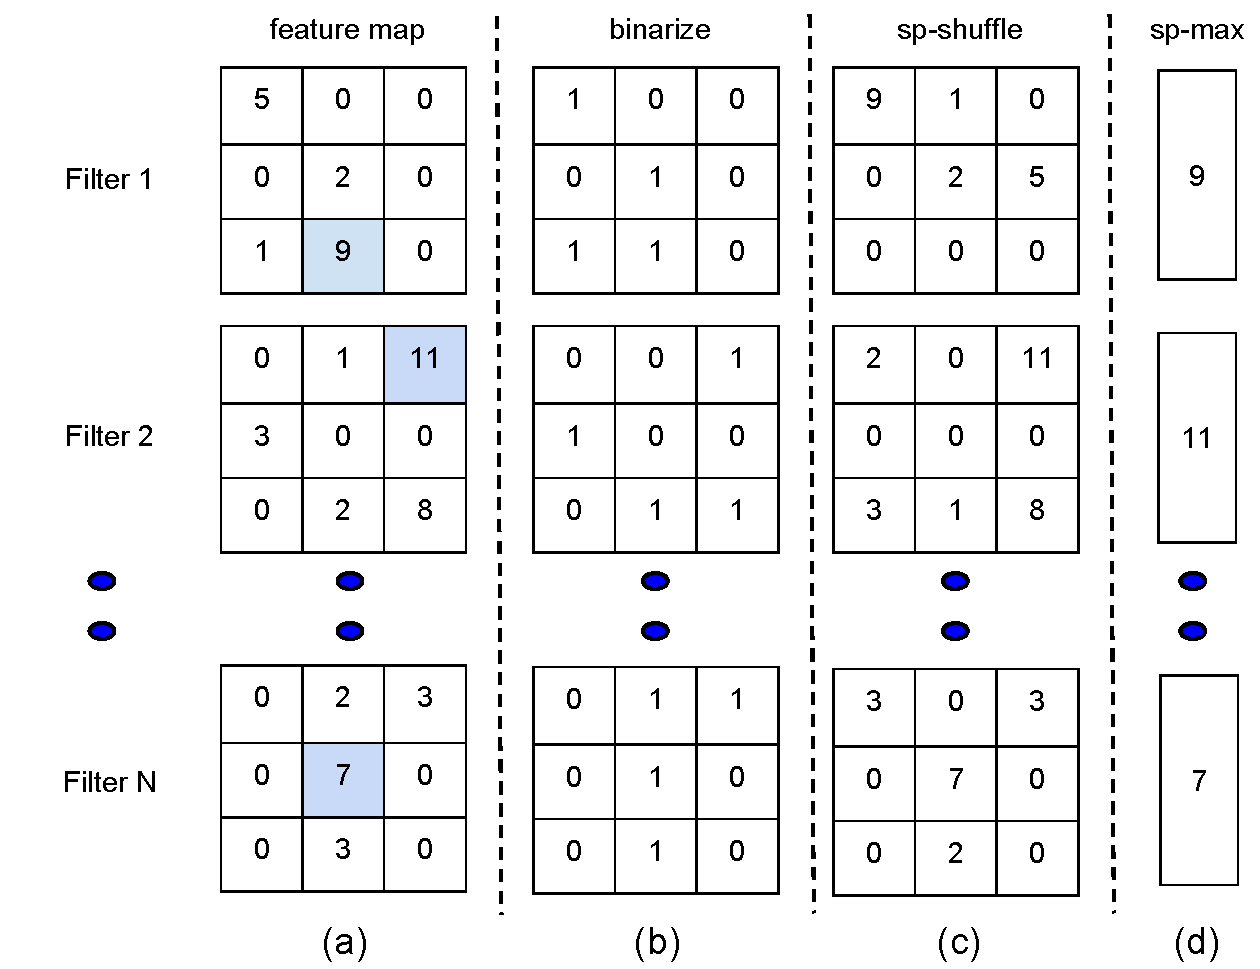
\includegraphics[height=6.5cm]{images/ablation.pdf}
\caption{Illustrations of ablations of feature activation spatial and magnitude information.
See Sections \ref{sub:imp-mag} and \ref{sub:imp-loc} for details.}
\label{fig:features}
\end{figure}

\subsection{How important is filter response magnitude?}
\label{sub:imp-mag}
\setlength{\tabcolsep}{4pt}
\begin{table}[t!]
\begin{center}
%\caption{Percentage non-zeros (sparsity) in filter responses of various layers of CNN.}
\caption{Percentage non-zeros (sparsity) in filter responses of CNN.}
\label{table:sparse}
\scalebox{1}{
\begin{tabular}{c|c|c|c|c|c|c}
conv-1 & conv-2 & conv-3 & conv-4 & conv-5 & fc-6 & fc-7 \\
\hline
$87.5 \pm 4.4$ & $44.5 \pm 4.4$ & $31.8 \pm 2.4$ & $32.0 \pm 2.7$ & $27.7 \pm 5.0$ & $16.1 \pm 3.0$ & $21.6 \pm 4.9$ \\
\end{tabular}}
\end{center}
\end{table}
\setlength{\tabcolsep}{1.4pt}

We can asses the importance of magnitude by setting each filter response $x$ to 1 if $x > 0$ and to $0$ otherwise. This binarization is performed prior to using the responses as features in a linear classifier and leads to loss of information contained in the magnitude of response while still retaining information about which filters fired and where they fired. 
In Tables \ref{table:class-ablation} and \ref{table:det-ablation} we show that binarization leads to a negligible performance drop for both classification and detection. 

For the fully-connected layers (fc-6 and fc-7) PASCAL-CLS performance is nearly identical before and after binarization.
This is a non-trivial property since transforming traditional computer vision features into short (or sparse) binary codes is an active research area. Such codes are important for practical applications in large-scale image retrieval and mobile image analysis \cite{gong2011iterative,weiss2009spectral}. Here we observe that sparse binary codes come essentially ``for free'' when using the representations learned in the fully-connected layers.

\subsection{How important is response location?}
\label{sub:imp-loc}
Now we remove spatial information from filter responses while retaining information about their magnitudes. We consider two methods for ablating spatial information from features computed by the convolutional layers (the fully-connected layers do not contain \emph{explicit} spatial information).

The first method (``sp-max'') simply collapses the $p \times p$ spatial map into a single value per feature channel by max pooling. The second method (``sp-shuffle'') retains the original distribution of feature activation values, but scrambles spatial correlations between columns of feature channels. To perform sp-shuffle, we permute the spatial locations in the $p \times p$ spatial map. This permutation is performed independently for each network input (i.e., different inputs undergo different permutations). Columns of filter responses in the same location move together, which preserves correlations between features within each (shuffled) spatial location. These transformations are illustrated in Figure \ref{fig:features}.

For image classification, damaging spatial information leads to a large difference in performance between original and spatially-ablated conv-1 features, but with a gradually decreasing difference for higher layers (Table \ref{table:class-ablation}). 
In fact, the performance of conv-5 after sp-max is close to the original performance. 
This indicates that a lot of information important for classification is encoded in the activation of the filters and not necessarily in the spatial pattern of their activations.
Note, this observation is not an artifact of small number of classes in PASCAL-CLS. On ImageNet validation data, conv-5 features and conv-5 after sp-max result into accuracy of 43.2 and 41.5 respectively. 
However, for detection sp-max leads to a large drop in performance. 
This may not be surprising since detection requires spatial information for precise localization.

\setlength{\tabcolsep}{4pt}
\begin{table}[t!]
\begin{center}
%\caption{Location and magnitude ablation study on PASCAL-CLS.}
\caption{Effect of location and magnitude feature ablations on PASCAL-CLS.}
\label{table:class-ablation}
\begin{tabular}{lccccc}
\noalign{\smallskip}
layer & no ablation (mAP) & binarize (mAP) & sp-shuffle (mAP) & sp-max (mAP) \\
\noalign{\smallskip}
\hline
\noalign{\smallskip}
conv-1 & $25.1 \pm 0.5$ & $17.7 \pm 0.2$ & $15.1 \pm 0.3$ & $25.4 \pm 0.5$  \\ 
conv-2 & $45.3 \pm 0.5$ & $43.0 \pm 0.6$ & $32.9 \pm 0.7$ & $40.1 \pm 0.3$  \\ 
conv-3 & $50.7 \pm 0.6$ & $47.2 \pm 0.6$ & $41.0 \pm 0.8$ & $54.1 \pm 0.5$  \\
conv-4 & $54.5 \pm 0.7$ & $51.5 \pm 0.7$ & $45.2 \pm 0.8$ & $57.0 \pm 0.5$  \\
conv-5 & $65.6 \pm 0.6$ & $60.8 \pm 0.7$ & $59.5 \pm 0.4$ & $62.5 \pm 0.6$  \\
fc-6   & $71.7 \pm 0.3$ & $71.5 \pm 0.4$ &  -             &  -   \\
fc-7   & $74.1 \pm 0.3$ & $73.7 \pm 0.4$ &  -             &  -   \\
\end{tabular}
\end{center}
\end{table}
\setlength{\tabcolsep}{1.4pt}

\setlength{\tabcolsep}{4pt}
\begin{table}[t!]
\begin{center}
\caption{Effect of location and magnitude feature ablations on PASCAL-DET.}
\label{table:det-ablation}
\scalebox{1.0}{
\begin{tabular}{l|c|c|c}
& no ablation (mAP) & binarize (mAP) & sp-max (mAP) \\
\hline
conv-5 & 47.6 & 45.7 & 25.4 
\end{tabular}}
\end{center}
\end{table}
\setlength{\tabcolsep}{1.4pt}

\begin{comment}
\setlength{\tabcolsep}{1pt}
\begin{table}[t!]
\begin{center}
\caption{Ablation study on PASCAL-DET using conv-5 features. Feature binarization leads to negligible drop in performance whereas as sp-max causes a large drop.}
\label{table:det-ablation}
\scalebox{0.70}{
\begin{tabular}{l|cccccccccccccccccccc||c}
\noalign{\smallskip}
& aero & bike & bird & boat & bottle & bus & car & cat & chair & cow & table & dog & horse & mbike & person & plant & sheep & sofa & train & tv & mAP \\
\noalign{\smallskip}
\hline
conv-5  & 57.8 & 63.9 & 38.8 & 28.0 & 29.0 & 54.8 & 66.9 & 51.3 & 30.5 & 52.1 & 45.2 & 43.2 & 57.3 & 58.8 & 46.0 & 27.2 & 51.2 & 39.3 & 53.3 & 56.6 & 47.6 \\
binarize & 57.9 & 61.3 & 32.6 & 24.7 & 27.5 & 55.0 & 64.7 & 49.8 & 25.3 & 47.4 & 44.5 & 40.3 & 54.6 & 56.4 & 43.6 & 27.1 & 48.4 & 41.6 & 54.3 & 57.6 & 45.7 \\
sp-max & 35.0 & 38.7 & 17.3 & 16.9 & 13.9 & 38.4 & 45.6 & 29.2 & 11.0 & 20.2 & 21.0 & 23.5 & 27.2 & 37.0 & 20.5 & 7.0 & 30.3 & 13.4 & 28.3 & 32.9 & 25.4 \\
\noalign{\smallskip}
\end{tabular}}
\end{center}
\end{table}
\setlength{\tabcolsep}{1.4pt}
\end{comment}

\section{Are there grandmother cells in CNNs?}
\label{sec:grand-mother}
Neuroscientists have conjectured that cells in the human brain which only respond to very specific and complex visual stimuli (such as the face of one's grandmother) are involved in object recognition.
These neurons are often referred to as \emph{grandmother cells} (GMC) \cite{Barlow,Grandmother}. Proponents of artificial neural networks have shown a great interest in reporting the presence of GMC-like filters for specific object classes in their networks (see, for example, the cat filter reported in \cite{GoogleCat}). More recently, for understanding feature representations in CNNs, \cite{Simonyan,DeConv} presented methods for finding locally optimal visual inputs for individual filters.
%These methods isolate individual inputs that activate a filter, but do not characterize the \emph{distribution} of images that cause an individual filter to fire above a certain threshold. \todo{make this argument clearer}.
These methods only find the best, or in some cases top-$k$, visual inputs that activate a filter, but do not characterize the \emph{distribution} of images that cause an individual filter to fire above a certain threshold. For example, if it is found that the top-10 visual inputs for a particular filter are cats, it remains unclear what is the response of the filter to other images of a cat.
A GMC filter for the \emph{cat} class, is one that fires strongly on \emph{all} cats and nothing else.
%If, for example, we wish to see if the network contains a GMC filter for the \emph{cat} class, then we should look for a particular filter that fires strongly on all cats and nothing else.
This criteria can be expressed as a filter that has high \emph{precision} and high \emph{recall}.
That is, a GMC filter for class $C$ is a filter that has a high average precision (AP) when tasked with classifying inputs from class $C$ versus inputs from all other classes.

%Mathematically, this computation is expressed as finding the set of images $\mathcal{I}$ which maximally activate a single feature (i.e. find $i \in \mathcal{I}$ s.t. Feature-score(i) $\geq th$ $\forall i $, where $th$ is a threshold value). The distribution of class labels associated with this set of images ($\mathcal{I}$), defines the \textit{precision} of the feature. However, this distribution does not account for the \textit{recall}.  The presence/absence of GMC is a scientifically interesting question to pursue, but for recognition, we require features with both high precision and high recall. Consequently, we argue that if the goal is object recognition, then GMC for a particular object class should be interpreted as features with high AP and not just high precision. 
 
Further, the notion of GMC-like features is related to standard feature encodings for image classification.
Prior to the work of \cite{Kriz}, the dominant approaches for image and scene classification were based on either representing images as a bag of local descriptors (BoW), such as SIFT (e.g., \cite{lazebnik2006beyond}), or by first finding a set of mid-level patches \cite{Blocks,Mid1} and then encoding images in terms of them. 
The problem of finding good mid-level patches is often posed as a search for a set of high-recall discriminative templates. 
In this sense, mid-level patch discovery is the search for a set of GMC templates. 
The low-level BoW representation, in contrast, is a \emph{distributed code} in the sense that a single feature by itself is not discriminative, but a group of features taken together is.
This makes it interesting to investigate the nature of mid-level CNN features such as conv-5. 

First, we address the question of finding GMC filters by computing the AP of individual filters (Section \ref{sub:class-specific-unit}). Next, we measure how distributed are the feature representations (Section \ref{sub:how-many}). For both experiments we use features from layer conv-5, which consists of responses of 256 filters in a $6\times 6$ spatial grid. Using max pooling, we collapse the spatial grid into a 256-D vector, so that for each filter we have a single response per image (in Section \ref{sub:imp-mag} we show that this transformation causes only a small drop in task performance).

%The output of conv-5 is the response of 256 filters in a $6\times 6$ spatial grid which we collapse into a 256-D vector using max-pooling (see section \ref{sub:imp-loc} for more details)

\setlength{\unitlength}{\linewidth}
\begin{figure}[t!]
\centering
%\subfloat{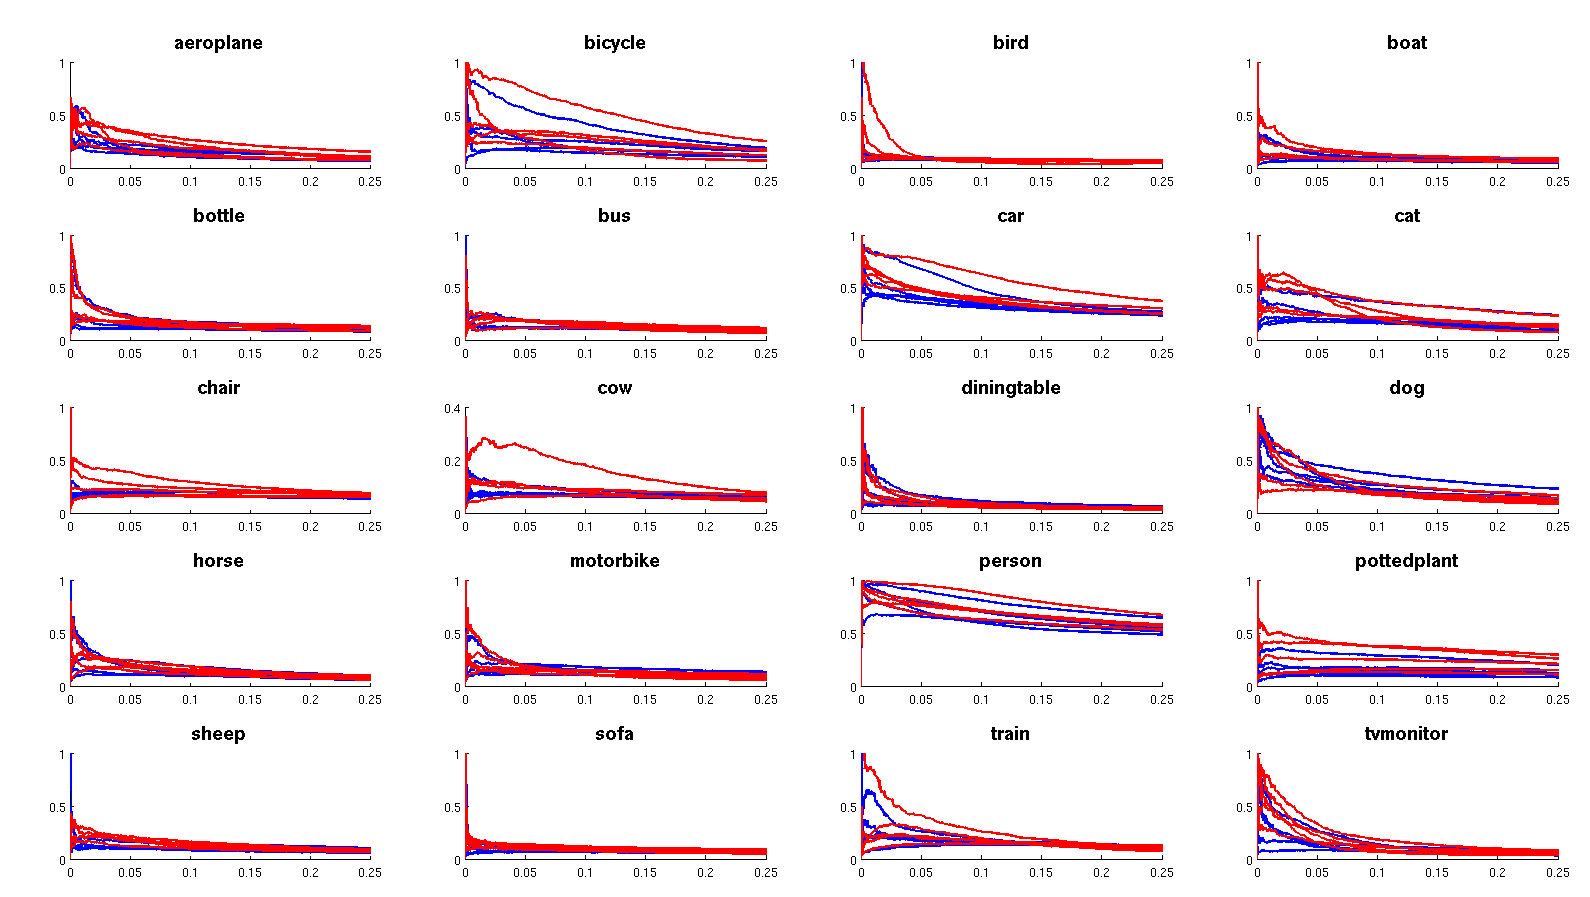
\includegraphics[scale=0.20]{images/gtbbox_pascal_prerec_pool5units.png}}
\begin{picture}(0.04,0.3)(0,0)
\put(0.0,0.20){\rotatebox{90}{\scriptsize{\textbf{Precision}}}}
\end{picture}
\subfloat{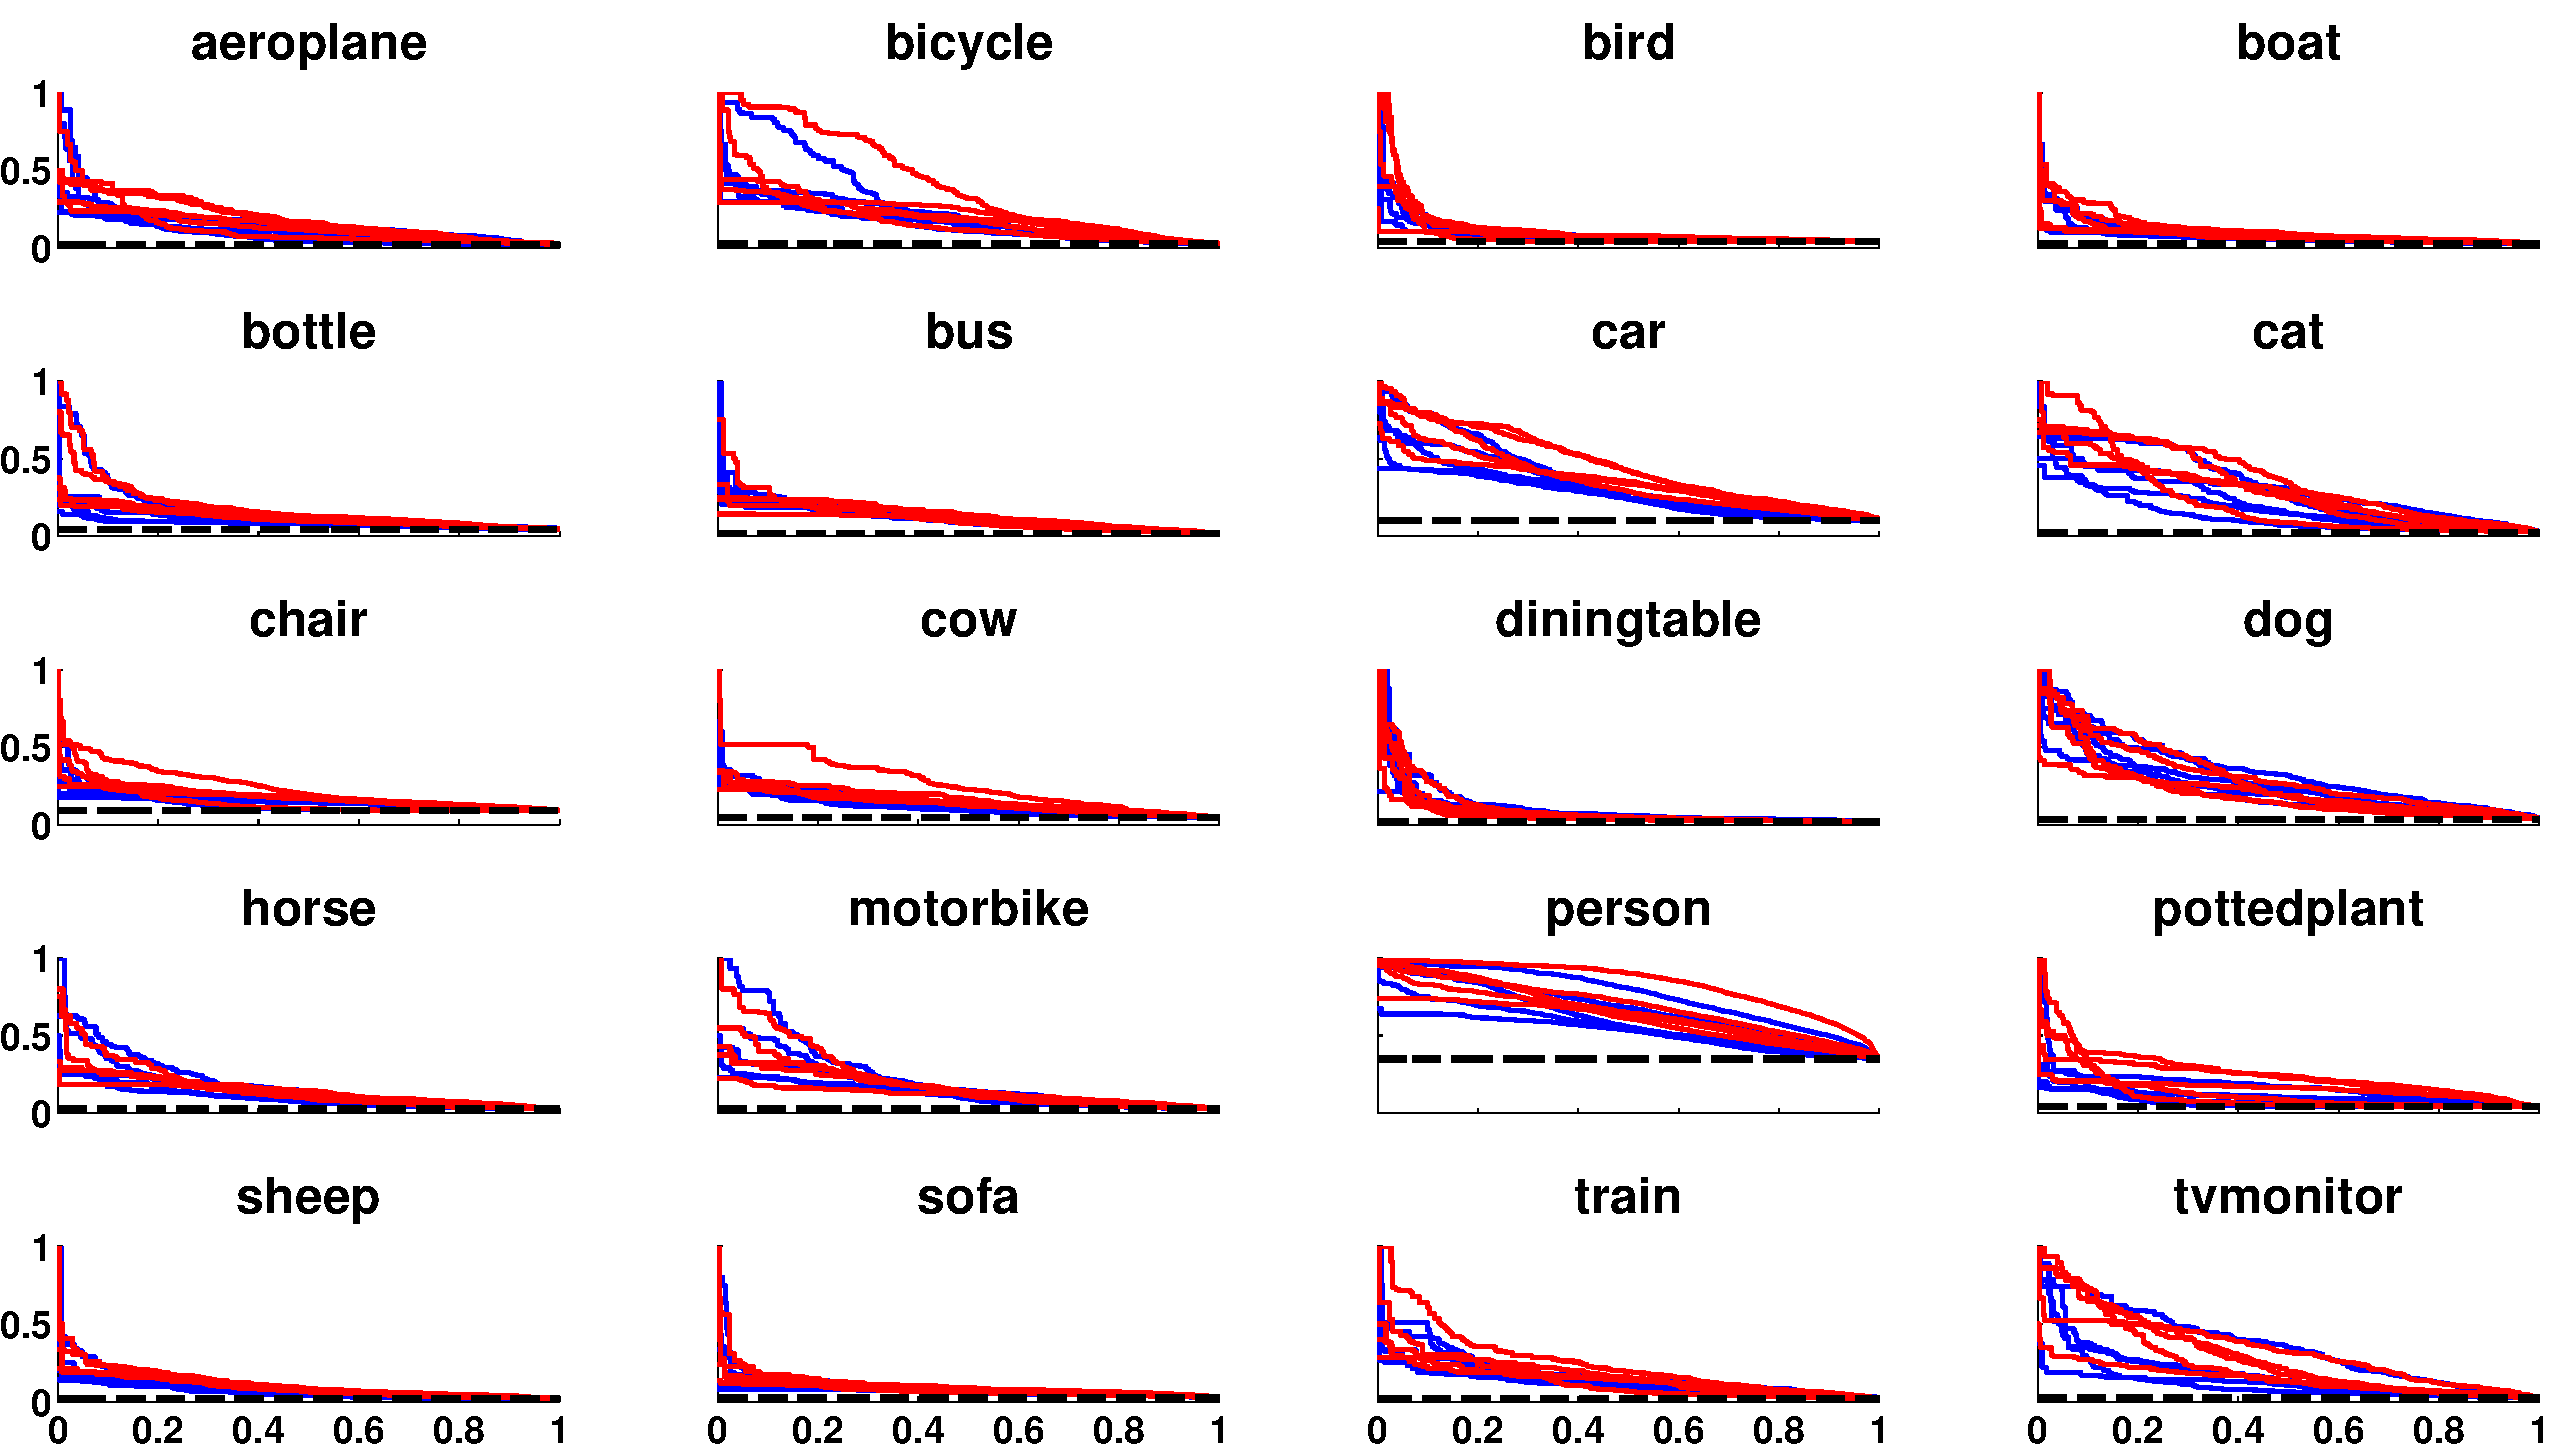
\includegraphics[width=0.93\linewidth]{images/pool5_ap_filters.pdf}} \vspace{0.4mm}
\begin{picture}(1.0,0.01)(0,0)
\put(0.50,0.0){{\scriptsize{\textbf{Recall}}}}
\end{picture}
\caption{The precision-recall curves for the top five (based on AP) conv-5 filter responses on PASCAL-DET-GT. Curves in red and blue indicate AP for fine-tuned and pre-trained networks, respectively. The dashed black line is the performance of a random filter. For most classes, precision drops significantly even at modest recall values. There are GMC filters for classes such as bicycle, person, car, cat.}
\label{fig:ap}
\end{figure}

\subsection{Finding Grandmother Cells}
\label{sub:class-specific-unit}
For each filter, its AP value is calculated for classifying images using class labels and filter response to images from PASCAL-DET-GT. Then, for each class we sorted filters in decreasing order of their APs. If GMC filters for this class exist, they should be the top ranked filters in this sorted list. The precision-recall curves for the top-five conv-5 filters are shown in Figure \ref{fig:ap}. We find that GMC-like filters exist for only for a few classes, such as bicycle, person, cars, and cats.


%\begin{figure}[t!]
%\centering
%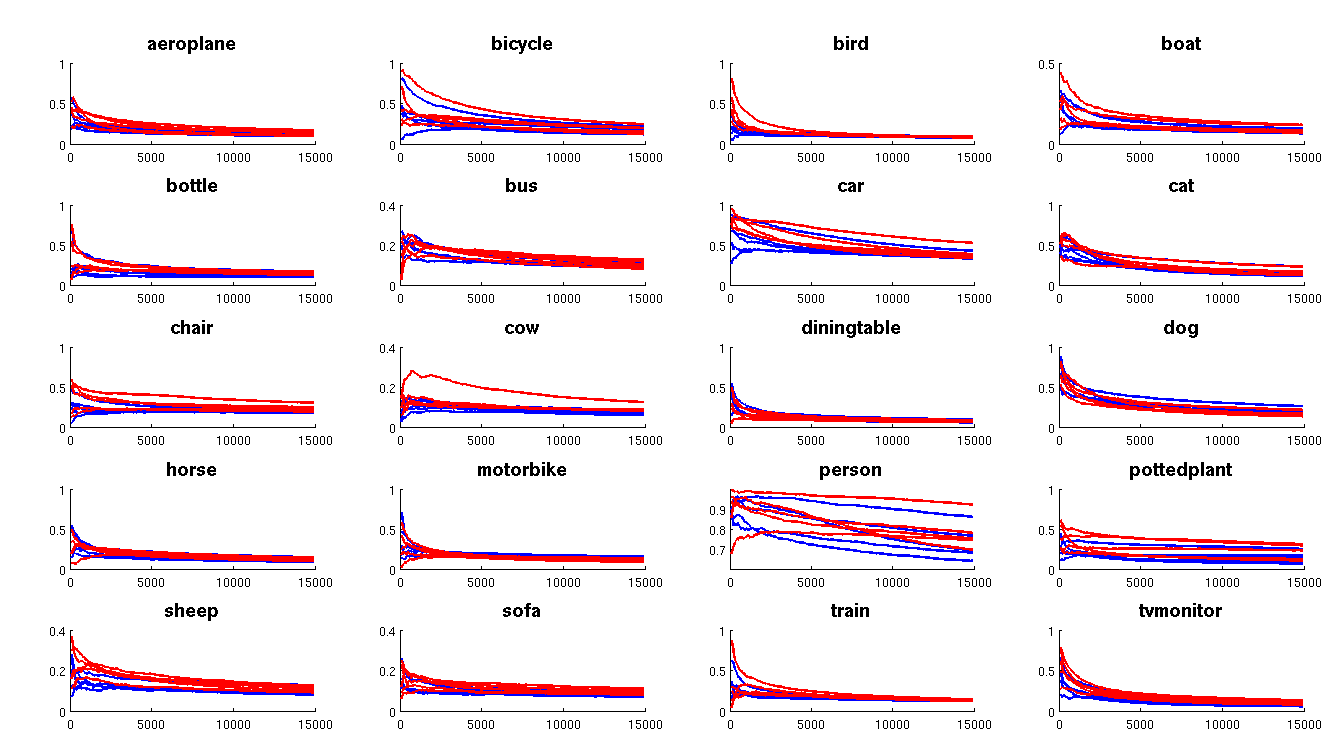
\includegraphics[scale=0.20]{images/prob_sel_dims_top5.png}
%\caption{This plot shows the precision curve for the top 5 most selective filters taken from Alex-Net (Blue) and FT-Net(Red) for all PASCAL classes. Y-axis is the precision and X-axis is number of examples.}
%\label{fig:prob-sel}
%\end{figure}

\subsection{How distributed are the feature representations?}
\label{sub:how-many}

%\begin{comment}
%\begin{figure}[t!]
%\centering
%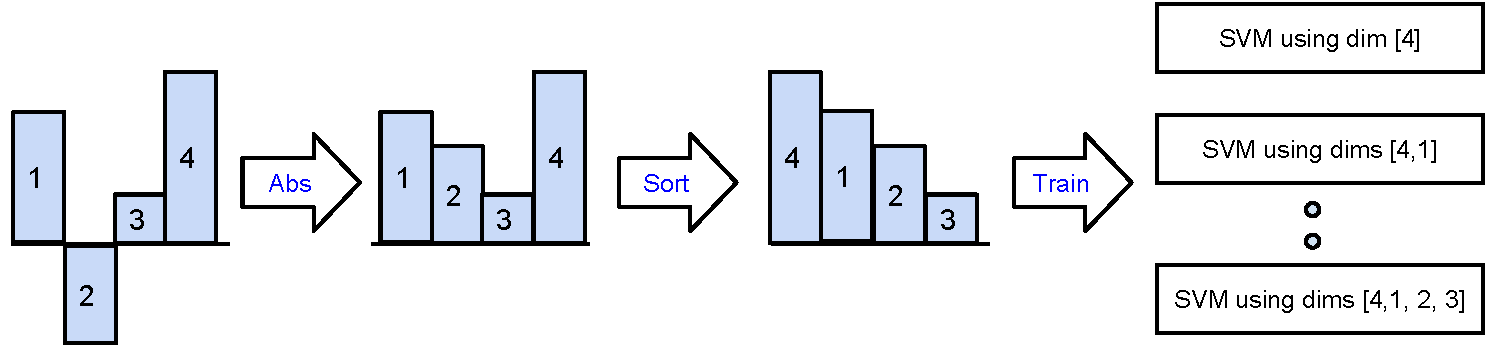
\includegraphics[scale=0.35]{images/how-many.pdf}
%\caption{Illustrating the greedy strategy used for selecting filters. First, linear SVM is trained to classify images of particular classes from 256-D conv-5 responses. The magnitudes of individual dimensions of the learnt SVM weight vectors are used as a proxy for determining the importance of each dimension. For the sake of clarity, this procedure is described using a 4-D weight vector shown on the extreme left (the numbers on each bar are the dimension). Firstly, we take the absolute value for each dimension and then sort the dimensions based on this value. Then, we chose the top k filters/dimensions from this ranked list to construct a subset of size k.}
%%\caption{Illustration of the greedy strategy used for selecting filters. For each class, a linear SVM is trained after ``sp-max'' feature transformation described in section \ref{sub:imp-loc} is applied. ``sp-max''  reduces conv-5 features into a 256-D vector, wherein each dimension corresponds to one of the 256 conv-5 filters. The magnitude of individual dimensions of the weight vector learned by SVM is used as a proxy for determining the importance of each dimension. For the sake of clarity, this procedure is described using a 4-D weight vector shown on the extreme left (the numbers on each bar are the dimension). Firstly, we take the absolute value for each dimension and then sort the dimensions based on this value. Then, we chose the top k filters/dimensions from this ranked list to construct a subset of size k.}
%\label{fig:sel-strategy}
%\end{figure}
%\end{comment}

In addition to visualizing the AP curves of individual filters, we measured the number of filters required to recognize objects of a particular class. 
%Feature selection was performed to construct nested subsets of filters, ranging from a single filter to all filters, using the greedy strategy described in Figure \ref{fig:sel-strategy}.\footnote{Filter subsets of size [1, 2, 3, 5, 10, 15, 20, 25, 30, 35, 40, 45, 50, 80, 100, 128, 256] were used.}
Feature selection was performed to construct nested subsets of filters, ranging from a single filter to all filters, using the following greedy strategy. First, separate linear SVMs were trained to classify object bounding boxes from PASCAL-DET-GT using conv-5 responses. 
For a given class, the 256 dimensions of the learnt weight vector ($w$) is in direct correspondence with the 256 conv-5 filters. We used the magnitude of the $i$-th dimension of $w$ to rank the importance of the $i$-th conv-5 filter for discriminating instances of this class. 
Next, all filters were sorted using these magnitude values. Each subset of filters was constructed by taking the top-$k$ filters from this list.\footnote{We used values of $k \in \{1, 2, 3, 5, 10, 15, 20, 25, 30, 35, 40, 45, 50, 80, 100, 128, 256\}$.} For each subset, a linear SVM was trained using only the responses of filters in that subset for classifying the class under consideration.

\setlength{\unitlength}{\linewidth}
\begin{figure}[t!]
\centering
%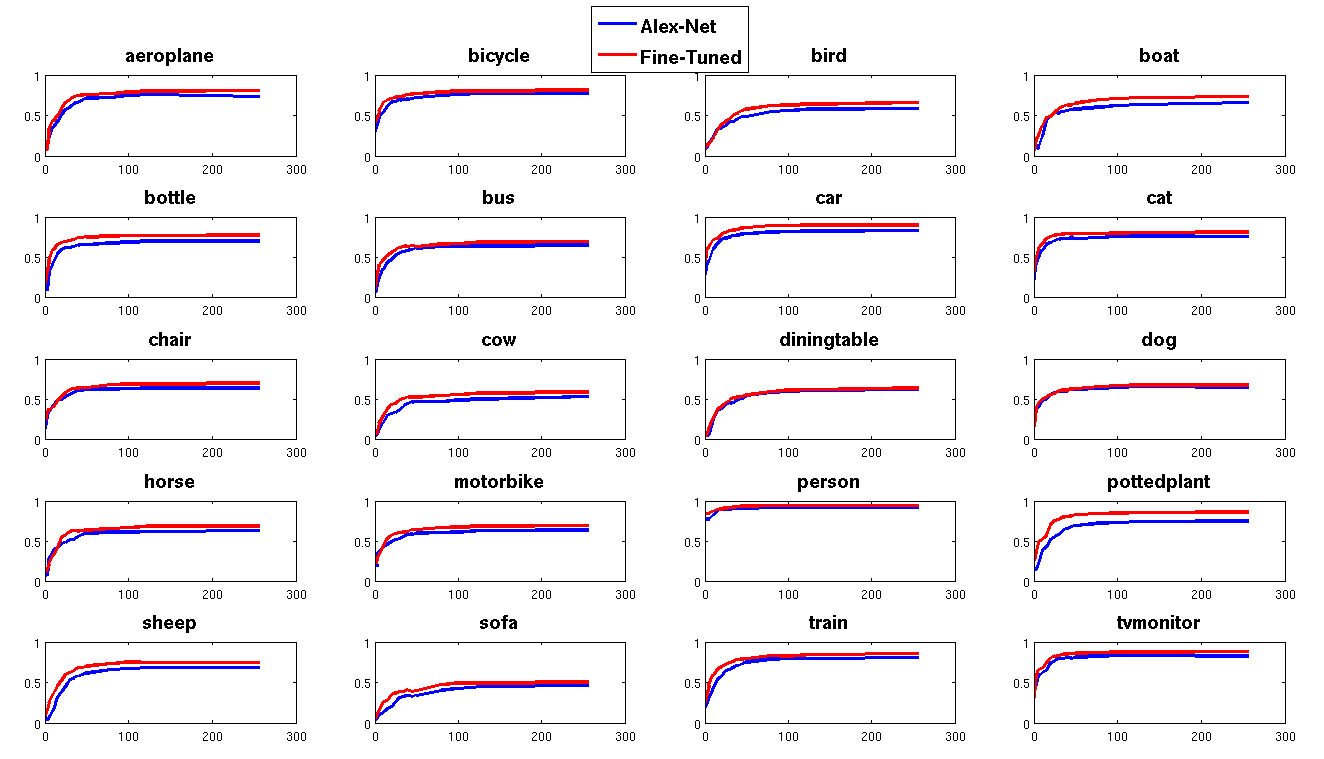
\includegraphics[height=6.5cm]{images/svm_seldims.png}
\begin{picture}(0.04,0.3)(0,0)
\put(0.0,0.06){\rotatebox{90}{\scriptsize{\textbf{Fraction of complete performance}}}}
\end{picture}
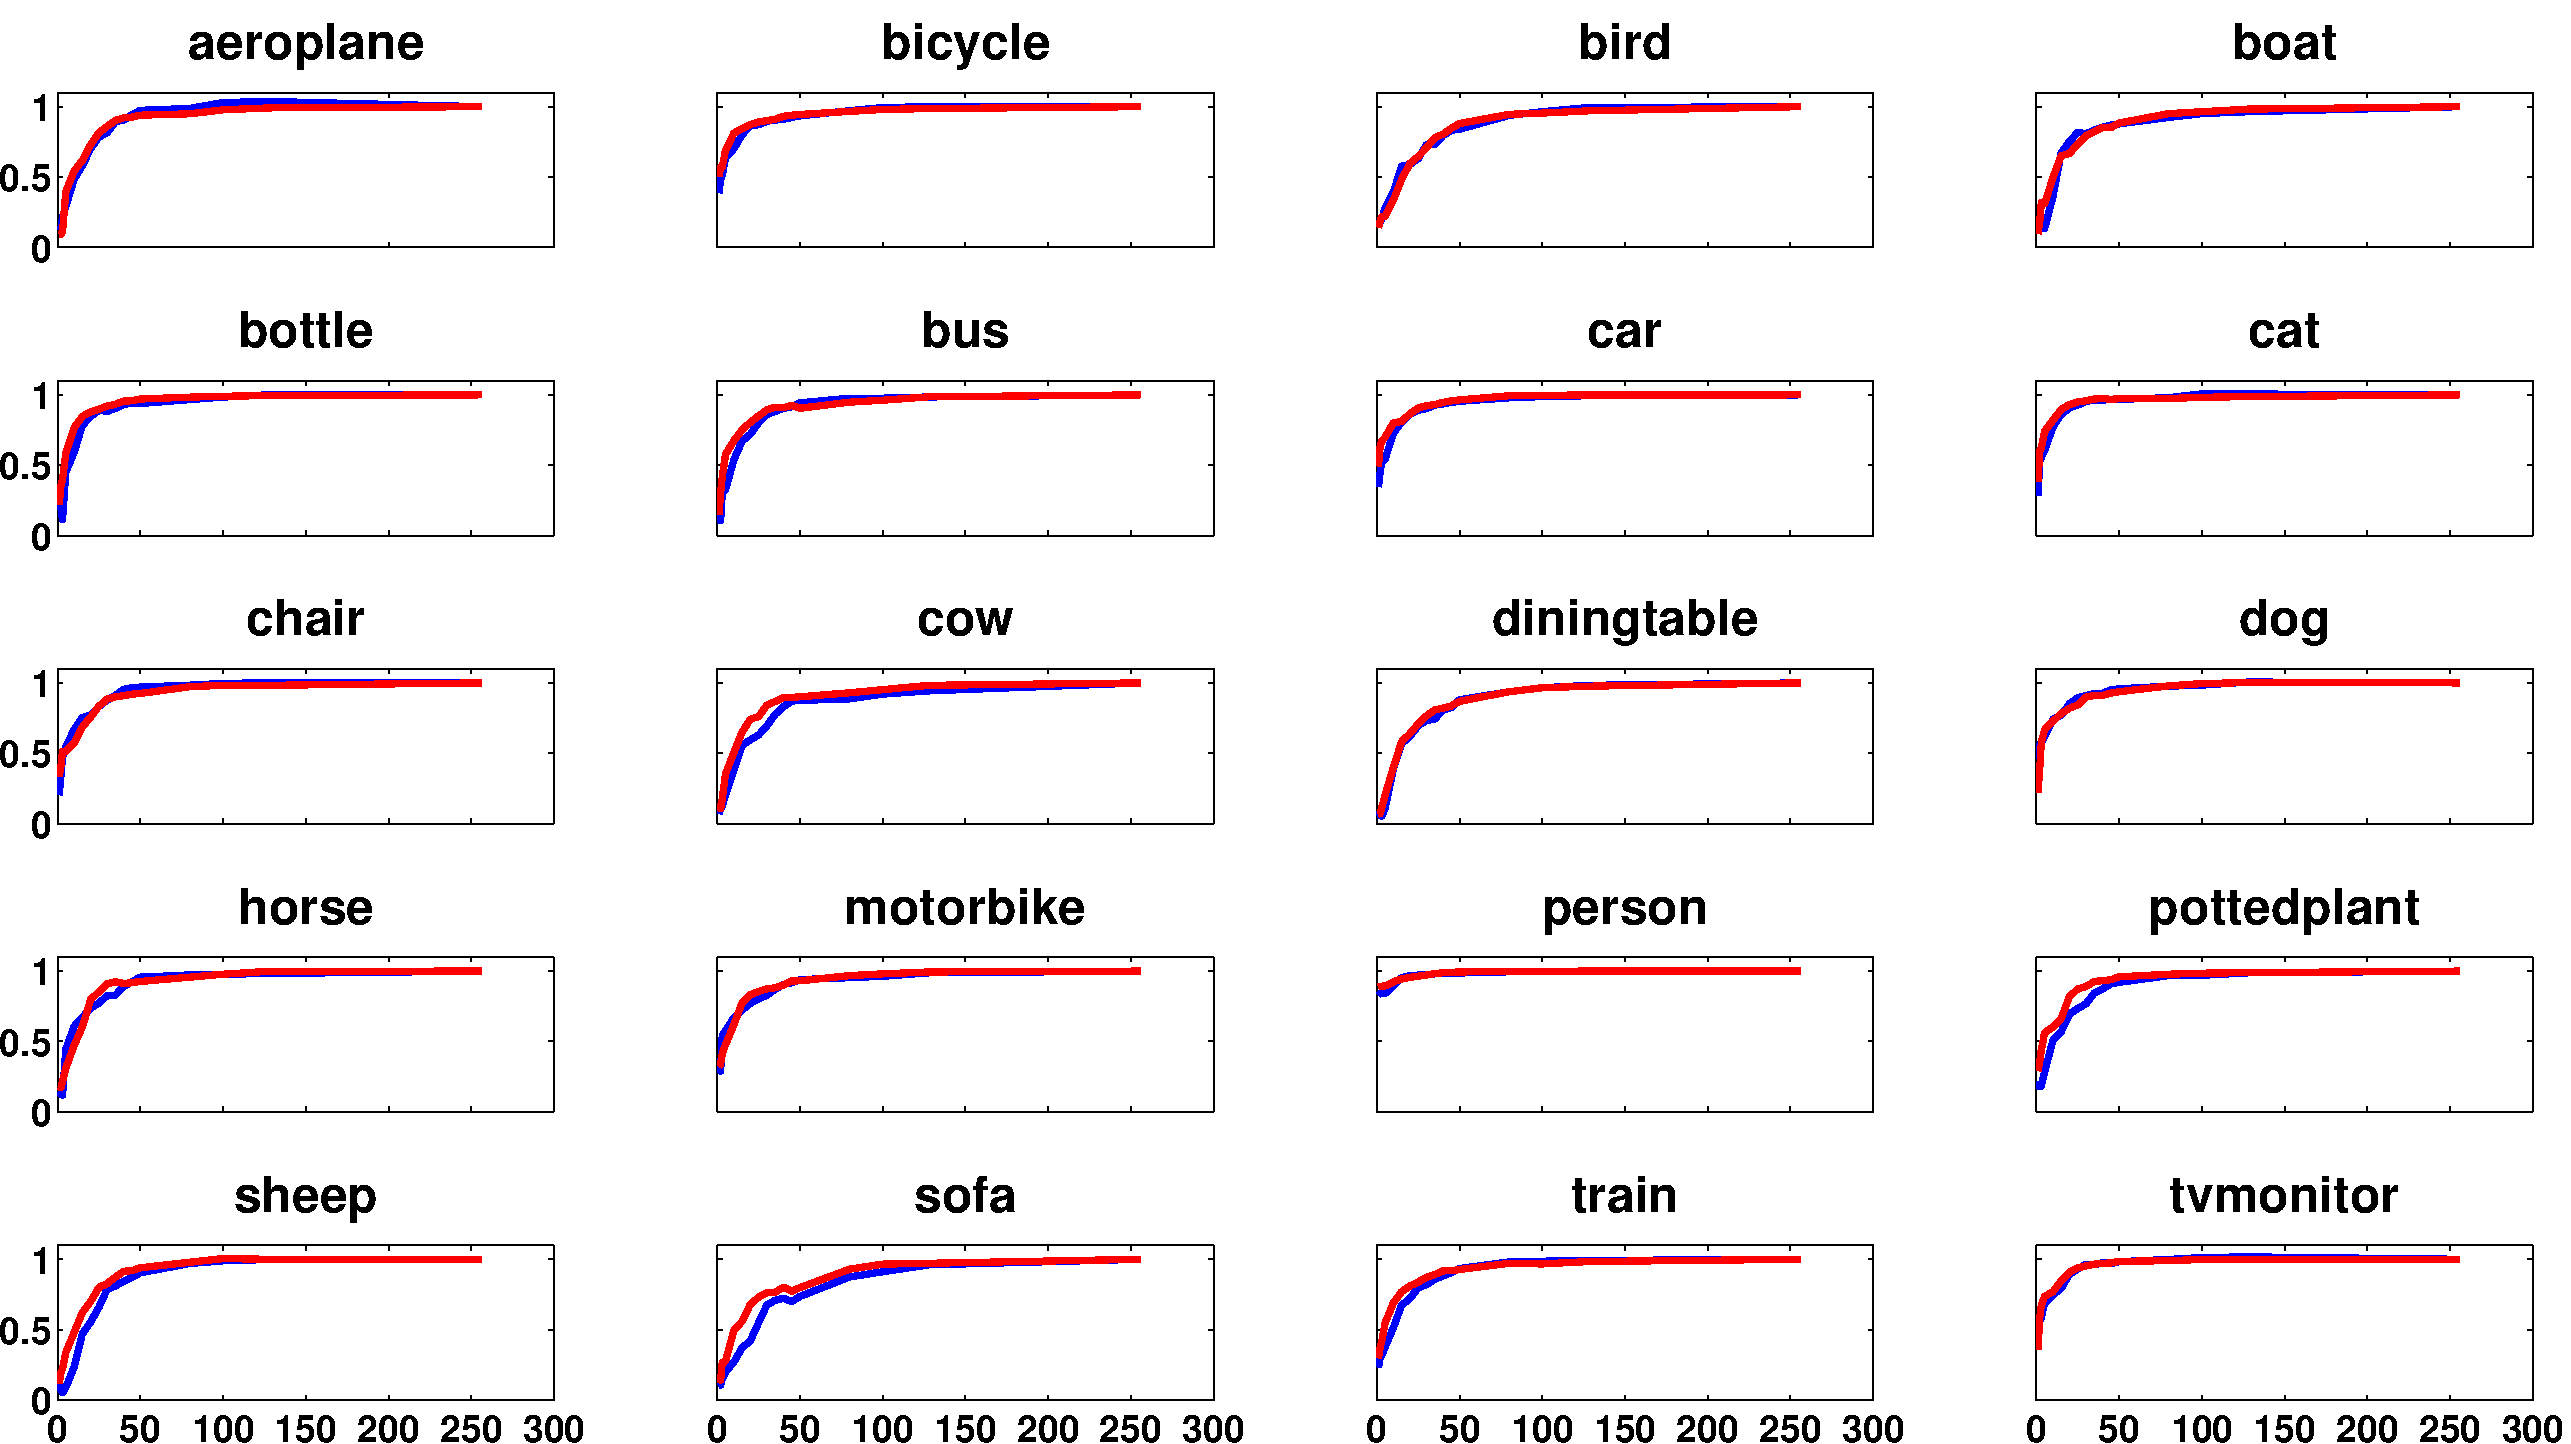
\includegraphics[width=0.93\linewidth]{images/pool5_spmax_num_svm_filters.pdf}
\begin{picture}(1.0,0.01)(0,0)
\put(0.40,0.0){{\scriptsize{\textbf{Number of conv-5 filters}}}}
\end{picture}
\caption{The fraction of complete performance on PASCAL-DET-GT achieved by conv-5 filter subsets of different sizes. Complete performance is the AP computed by considering responses of all the filters. Notice, that for a few classes such as \emph{person} and \emph{bicycle} only a few filters are required, but for most classes substantially more filters are needed, indicating a distributed code.}
\label{fig:svm-sel-dims}
\end{figure}  

\setlength{\tabcolsep}{1.1pt}
\begin{table}[t!]
\renewcommand{\arraystretch}{1.2}
\begin{center}
\caption{Number of filters required to achieve 50\%, 90\% of the complete performance on PASCAL-DET-GT using a CNN pre-trained on ImageNet and fine-tuned for PASCAL-DET using conv-5 features.}
\label{table:num-fil}
\resizebox{\linewidth}{!}{
\begin{tabular}{l|c||cccccccccccccccccccc}
\noalign{\smallskip}
& perf. & aero & bike & bird & boat & bottle & bus & car & cat & chair & cow & table & dog & horse & mbike & person & plant & sheep & sofa & train & tv \\
\hline
pre-train & 50\% & 15 & 3 & 15 & 15 & 10 & 10 & 3 & 2 & 5 & 15 & 15 & 2 & 10 & 3 & 1 & 10 & 20 & 25 & 10 & 2 \\ 
fine-tune & 50\% & 10 & 1 & 20 & 15 & 5 & 5 & 2 & 2 & 3 & 10 & 15 & 3 & 15 & 10 & 1 & 5 & 15 & 15 & 5 & 2 \\
\hline
pre-train & 90\% & 40 & 35 & 80 & 80 & 35 & 40 & 30 & 20 & 35 & 100 & 80 & 30 & 45 & 40 & 15 & 45 & 50 & 100 & 45 & 25 \\
fine-tune & 90\% & 35 & 30 & 80 & 80 & 30 & 35 & 25 & 20 & 35 & 50 & 80 & 35 & 30 & 40 & 10 & 35 & 40 & 80 & 40 & 20 \\
\end{tabular}
}
\end{center}
\end{table}
\setlength{\tabcolsep}{1.4pt}
  
The variation in performance with the number of filters is shown in Figure \ref{fig:svm-sel-dims}.
Table \ref{table:num-fil} lists the number of filters required to achieve 50\% and 90\% of the complete performance. For classes such as persons, cars, and cats relatively few filters are required, but for most classes around 30 to 40 filters are required to achieve at least 90\% of the full performance. This indicates that the conv-5 feature representation is distributed and there are GMC-like filters for only a few classes.
Results using layer fc-7 are presented in the the supplementary material.
We also find that after fine-tuning, slightly fewer filters are required to achieve performance levels similar to a pre-trained network. 

\begin{figure}[t!]
\centering
%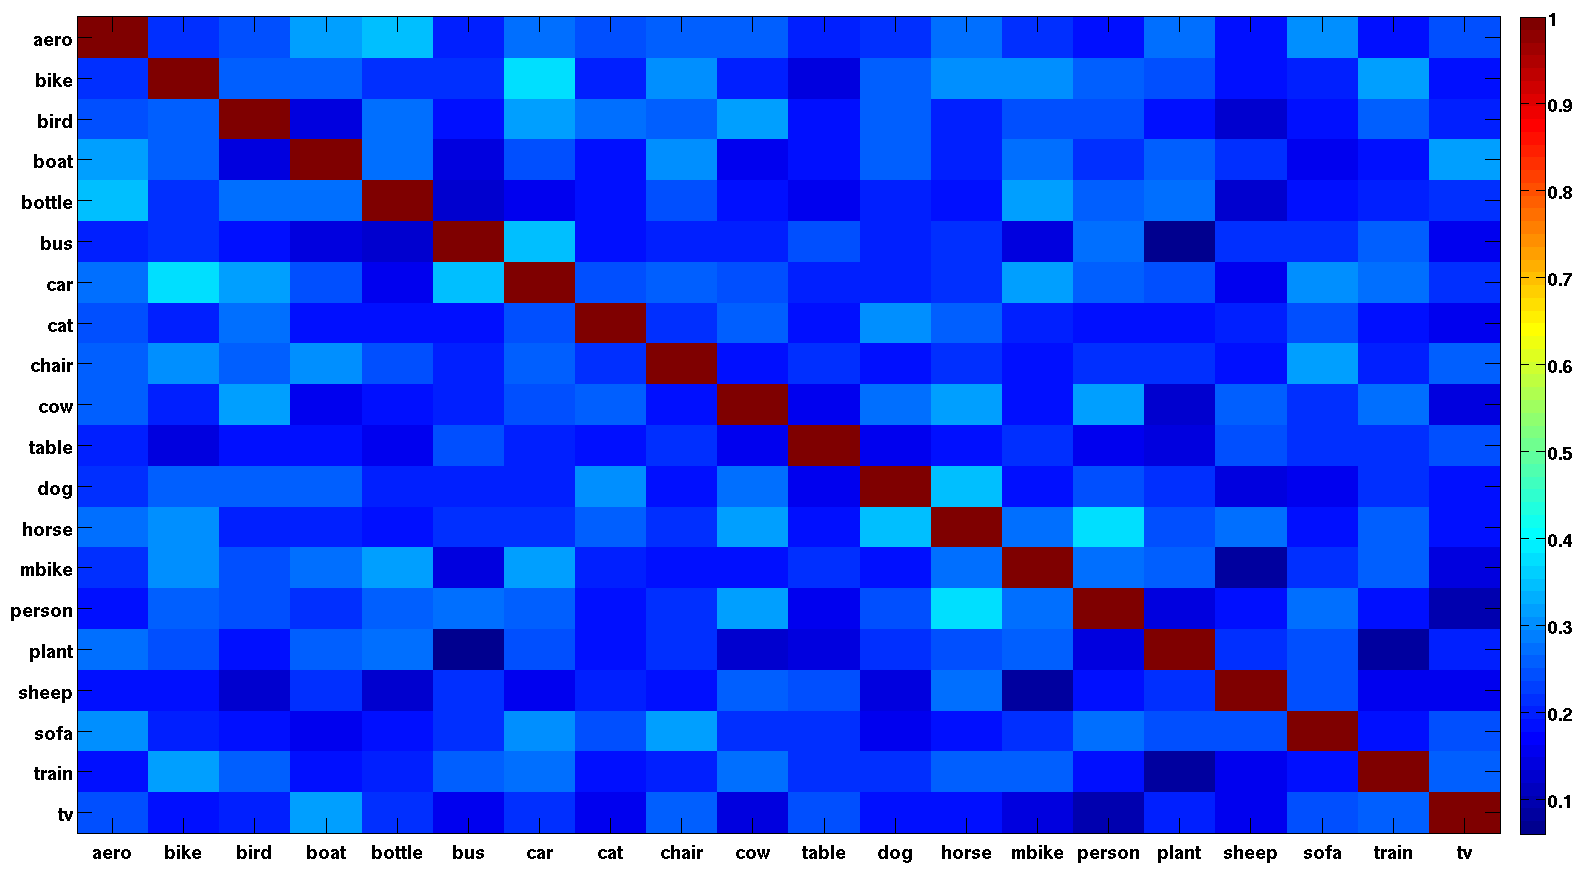
\includegraphics[width=1.0\linewidth]{images/ftNet_commonfilters.png}
%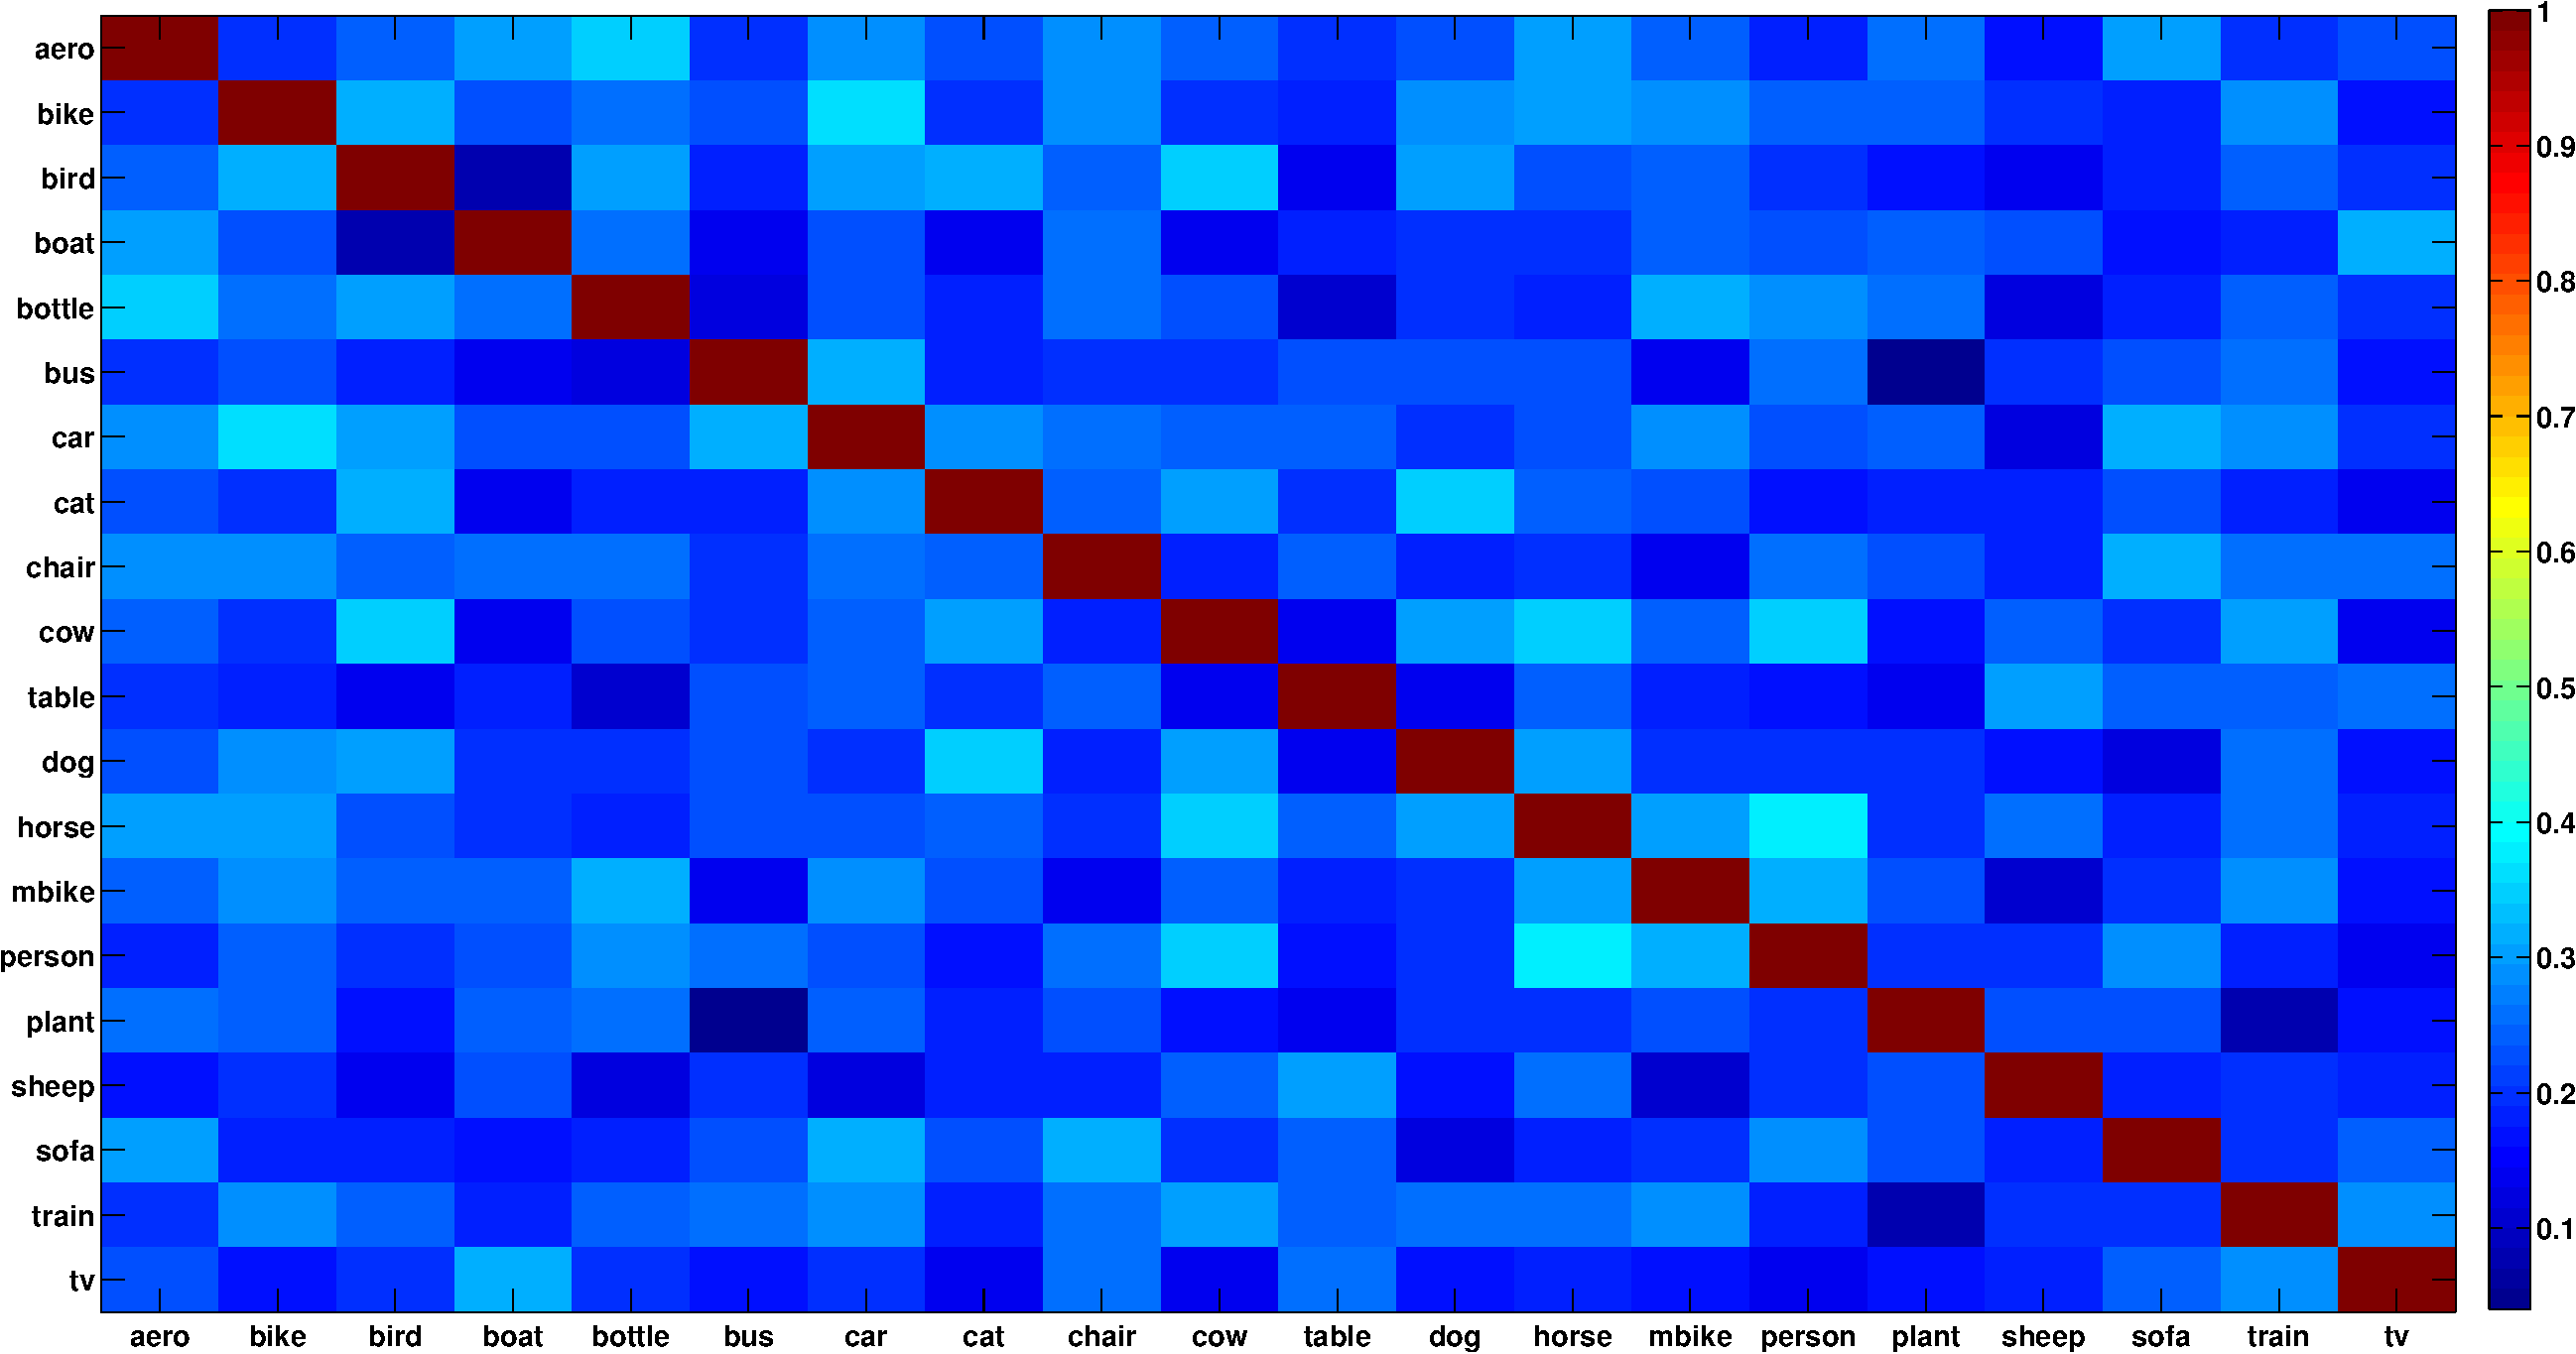
\includegraphics[width=1.0\linewidth]{images/FTNet_overlap.pdf}
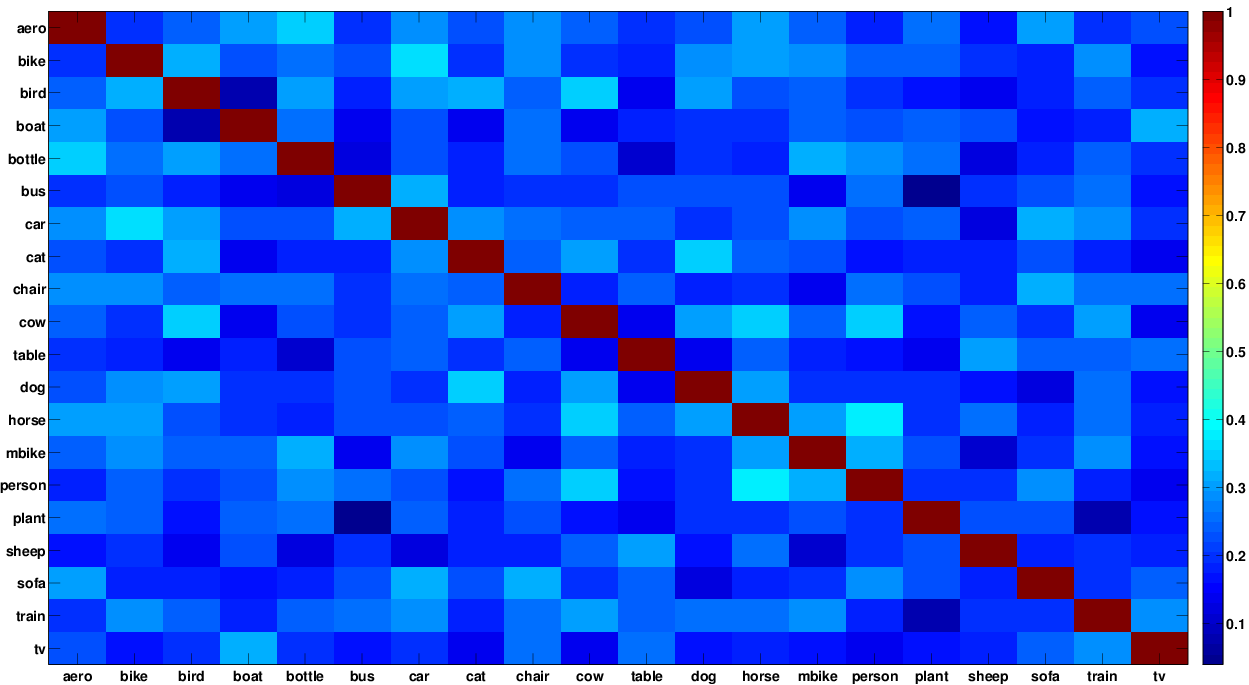
\includegraphics[width=1.0\linewidth]{images/ftNet.png}
\caption{The set overlap between the 50 most discriminative conv-5 filters for each class determined using PASCAL-DET-GT.
Entry $(i, j)$ of the matrix is the fraction of top-50 filters class $i$ has in common with class $j$ (Section \ref{sub:how-many}). Chance is 0.195. This is little overlap, but related classes are more likely to share filters.}
\label{fig:overlap}
\end{figure}

Next, we estimated the extent of overlap between the filters used for discriminating between different classes.
For each class $i$, we selected the 50 most discriminative filters (out of 256) and stored the selected filter indices in the set $S_i$.
The extent of overlap between class $i$ and $j$ was evaluated by $|S_i \cap S_j| / N$,
where $N = |S_i| = |S_j| = 50$. The results are visualized in Figure \ref{fig:overlap}. It can be seen that different classes use different subsets of conv-5 filters and there is little overlap between classes. This further indicates that intermediate representations in the CNN are distributed.
%and different sets of are used to distinguish between different classes. 


\section{What happens when a discriminatively pretrained network is finetuned?}
\label{sec:fine}
Finetuning a network is the process of slowly updating pre-learned parameters to minimize a target loss function for a new task at hand. Since, CNNs consist of large number of parameters they are prone to overfitting when trained on small datasets. Finetuning can be considered as a method of transfer learning and recent results from \cite{Rcnn, Decaf} presented a strong case for this methodology boosting performance. Although, unsupervised pretraining has been widely studied in the multilayer network literature \cite{AmitGeman, DeepPre}, there is no work analysing the effect of fine-tuning on different layers of a discriminatively trained multilayer convolutional networks.

We start our analysis by investigating how the discriminative capacity of different layers of the network changes as a result of finetuning. We measure discriminative capacity using the entropy of each layer  
%We start our analysis by investigating how the entropy of filters across different layers changes as a result of discriminative fine-tuning (see sec \ref{sub:fine-entropy}). Since, entropy of a filter can be evaluated at different threshold level of activations we propose the metric of Area under the Entropy curve (AuE) to judge changes in filter selectivity. Our main finding is that most of the learning during finetuning happens only in the top two fully connected layers. Motivated by this observation, we finetune networks for PASCAL detection and SUN-397 scene classification task by setting non-zero learning rates only in the top 2 layers (see sec\ref{sub:fine-fc-only}). We find this results in a negligible drop in performance and allows for moderate speed-ups in finetuning time. Other conclusions are presented in the sec \ref{sub:fine-discussion}.

\subsection{Entropy Analysis}
\label{sub:fine-entropy}
We compute the entropy  curve of each filter (using the method described in \ref{sub:def-ent}) for all layers of Alex-Net and FT-Net using the ground-truth bounding boxes taken from the VOC-2007 test-set. 

We use Area under this entropy curve (AuE) to quantify selectivity of each filter. The distribution of AuE for all filters across the seven layers of the CNN is illustrated in fig \ref{fig:fine-hist}. Next, in order to determine the overall change in a layer's tuning we use the Cumulative AuE (C-AuE) of filters sorted in decreasing order of their individual AuE's. We normalize this metric appropriately to account for different number of filters in different layers. We call this normalized C-AuE as MC-AuE. A lower value of MC-AuE means that a layer is more selective.  Fig \ref{fig:fine-entropy} plots MC-AuE as a function of fraction of filters in each layer. 

\begin{figure}[t!]
\centering
\subfloat{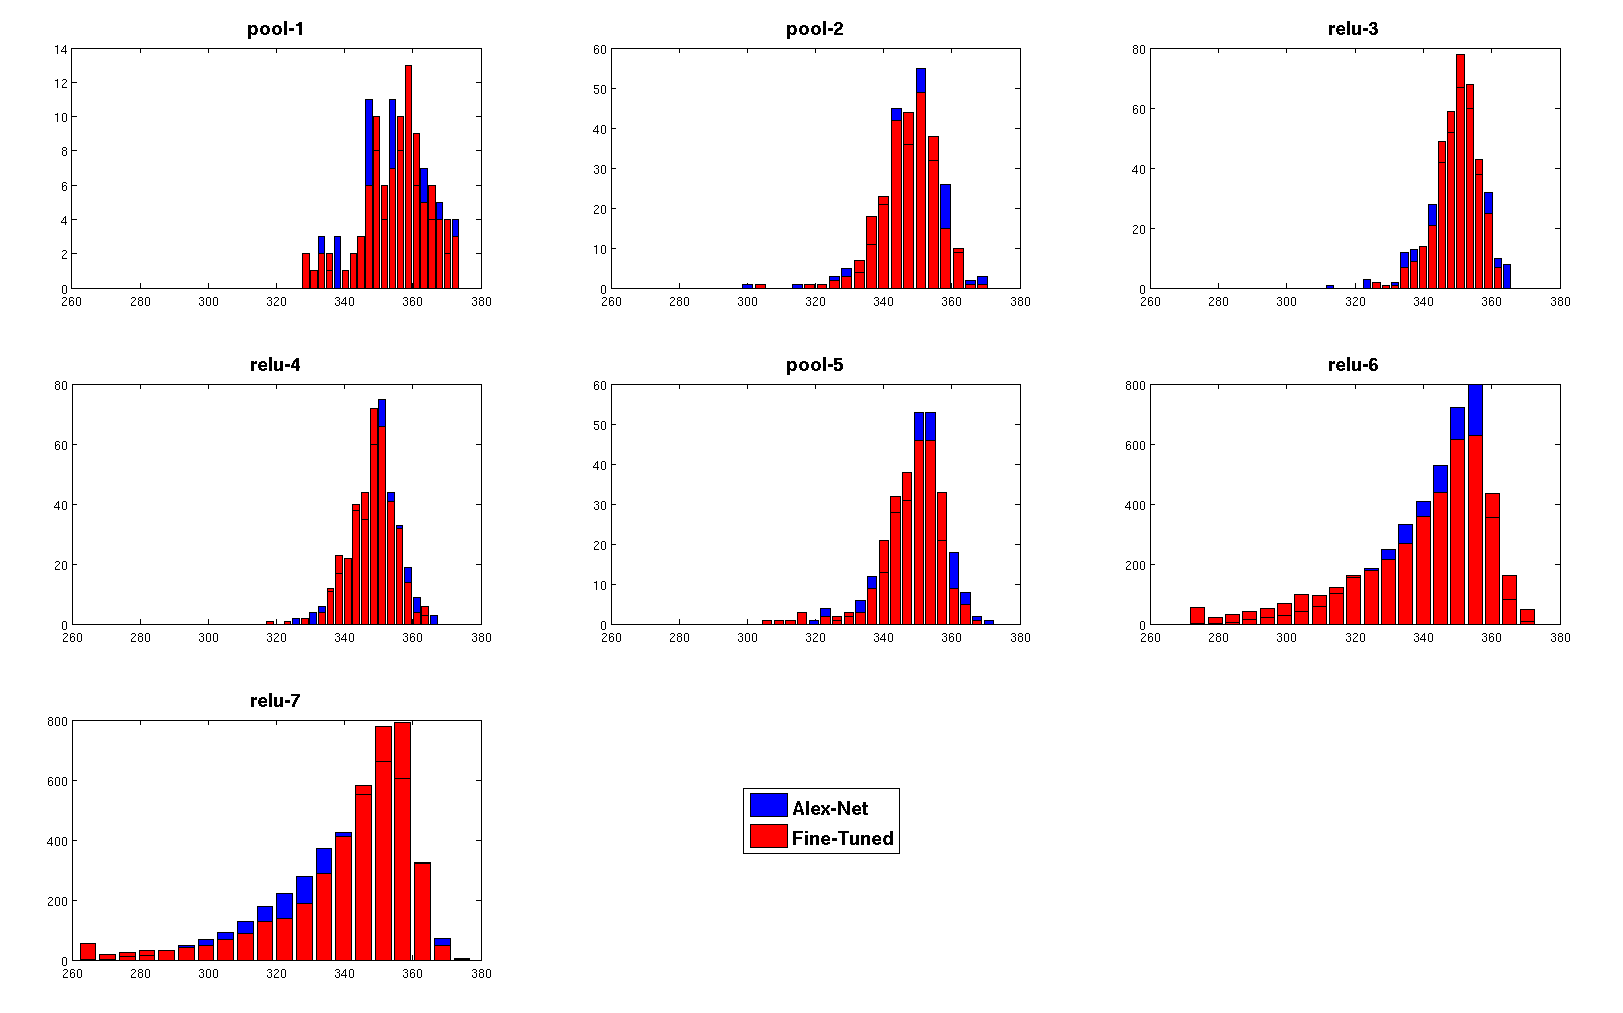
\includegraphics[height=6.5cm]{images/ent_hist.png}}
\caption{Distribution of AuE for different layers in Alex-Net and FT-Net. X-axis is the entropy and the Y-axis is the number of filters. Notice that the left tail for relu 6 and 7 becomes heavier after finetuning. This indicates that finetuning makes these filters more discriminative.}
\label{fig:fine-hist}
\end{figure}

\begin{figure}[t!]
\centering
\subfloat{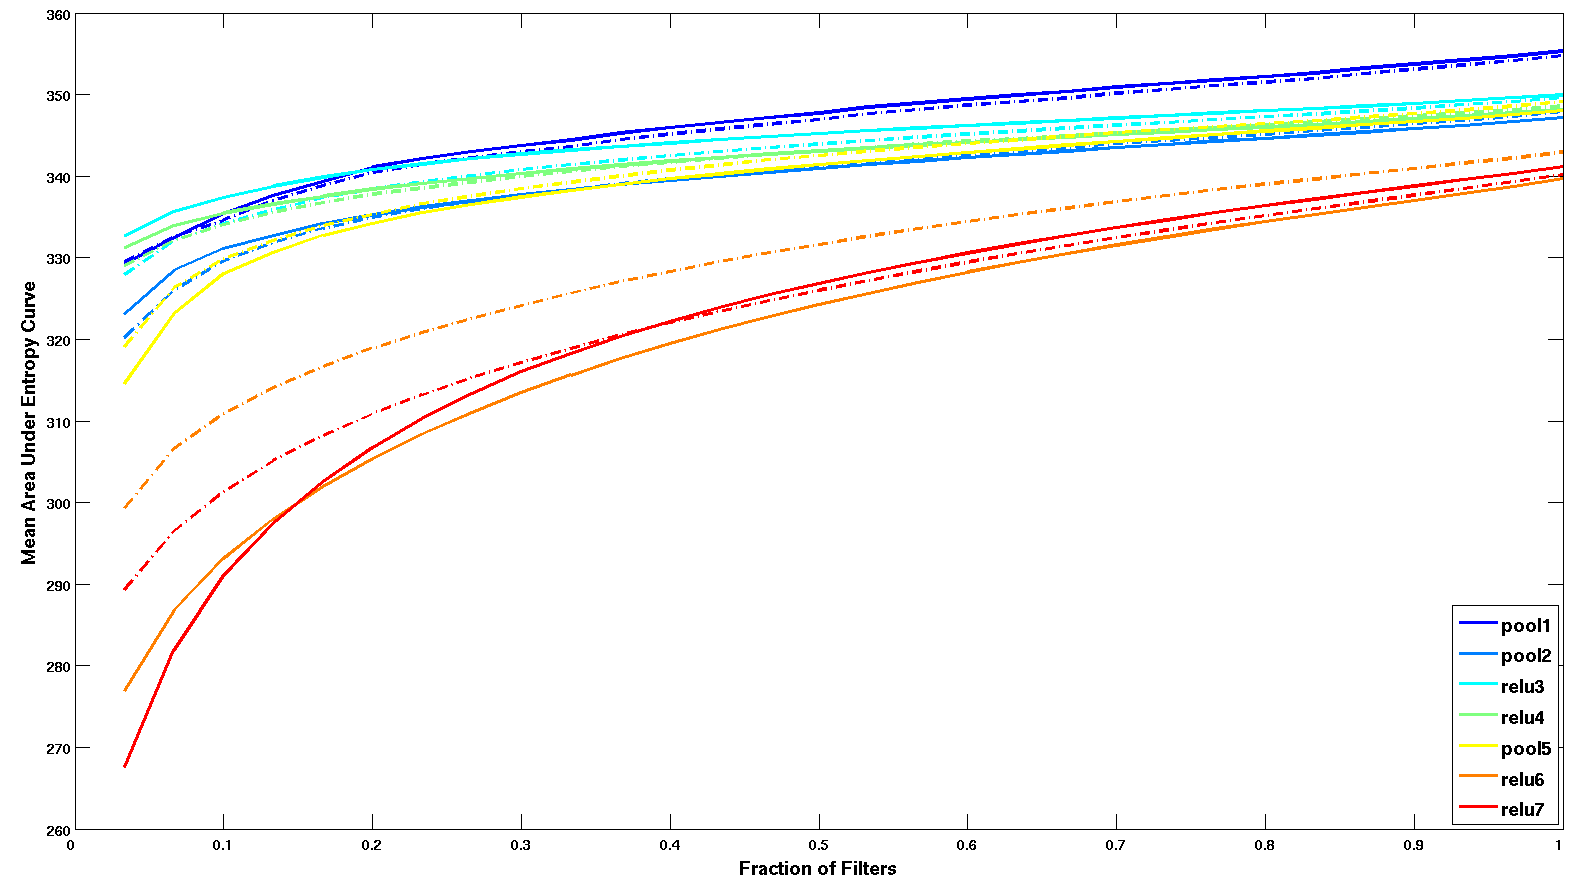
\includegraphics[scale=0.15]{images/entropy_variation.png}}
\caption{Mean Cumulative AuE plotted as fraction of filters (see sec \ref{sub:fine-entropy}). (Dash-Dot Line :Alex-Net, Solid Line: Fine-Tuned Network).}
\label{fig:fine-entropy}
\end{figure}

From figures \ref{fig:fine-hist} and \ref{fig:fine-entropy}, we draw 2 conclusions:
\begin{enumerate}
\item Although the entropy of filters decreases as we move to higher layers, the magnitude of change in entropy between layer 1 and layer 5 is small as compared to the change which happens when going from layer 5 to layer 6.
\item Finetuning mostly reduces the entropy of filters in the fully connected layers, there are small changes in layer 5 and negligible changes in other layers.
\end{enumerate} 

\subsection{Is finetuning only the fully-connected layers sufficient?}
\label{sub:fine-fc-only}
The observations made in \ref{sub:fine-entropy} indicate that finetuning the convolutional layers in the CNN may not be critical for achieving good-performance on novel datasets. We test this hypothesis on the 2 challenging tasks of object detection(PASCAL) and scene classification (SUN-397) by comparing the performance of a fully finetuned network with a network finetuned by only updating weights in the fully-connected (fc) layers. Our results are summarized in table \ref{table:fine-effect}.

\setlength{\tabcolsep}{2pt}
\begin{table}[t!]
\begin{center}
\caption{Comparison in performance on of Alex-Net, Finetuned Network(ft-net) and a network with only fc layers finetuned (fc-ft).}
\label{table:fine-effect}
\scalebox{0.85}{
\begin{tabular}{|l|cccc|cccc|cccc|}
\hline
Layer &  \multicolumn{4}{c|}{sun-397} & \multicolumn{4}{c|}{det VOC-2007-finetune} & \multicolumn{4}{c|}{det VOC-all-finetune} \\
\hline
  &    scratch & i-net & ft & fc-ft  & scratch & i-net & ft & fc-ft & scratch & i-net & ft & fc-ft\\
\hline
fc-7 & $40.2 \pm $ & $53.1 \pm 0.2$ & $56.8 \pm 0.2$ & $56.2 \pm 0.1$ & 40.7 & 45.5 & 54.1 & 53.3 & 52.3 & 53.1 & 56.0 & 59.2 \\ 
\hline
\end{tabular}}
\end{center}
\end{table}
\setlength{\tabcolsep}{1.4pt}

We find that indeed it is the case that the final performance in the detection setup only drops by 0.8 points and by 0.6 points for scene-classification. In our experiments we also noted accuracy of image classification on PASCAL is almost untouched by finetuning. This is suggestive of the fact finetuning is a task specific operation and finetuning for detection does not necessarily leads to an increase in classification performance, even though the classes and images are shared across PASCAL classification and detection challenges. 

\setlength{\tabcolsep}{1pt}
\begin{table}[t!]
\begin{center}
\caption{Evaluation of effect finetuning towards the task of object detection. (l5, l6, l7: layers 5, 6 and 7 of Alex Net)}
\label{table:det-fine}
\scalebox{0.75}{
\begin{tabular}{l|cccccccccccccccccccc||c}
\hline\noalign{\smallskip}
layer & aero & bike & bird & boat & bottle & bus & car & cat & chair & cow & table & dog & horse & mbike & person & plant & sheep & sofa & train & tv & mAP \\
\noalign{\smallskip}
\hline
l5 & 51.9 & 61.1 & 36.8 & 28.4 & 23.7 & 52.3 & 60.8 & 48.4 & 24.9 & 47.1 & 47.5 & 42.1 & 55.6 & 58.7 & 42.5 & 24.5 & 46.9 & 39.3 & 52.0 & 55.4 & 45.0 \\
l5-ft & 57.8 & 63.9 & 38.8 & 28.0 & 29.0&54.8&66.9&51.3 & 30.5 & 52.1 & 45.2 & 43.2 & 57.3 & 58.8 & 46.0 & 27.2 & 51.2 & 39.3 & 53.3 & 56.6 & 47.6 \\
\hline 
l6-ft &63.5 & 66.3 & 48.7 & 38.1 & 30.6 & 61.4 & 70.9 & 60.3 & 34.8 & 57.8 & 47.6 & 53.6 & 59.8 & 63.5 & 52.5 & 29.8 & 54.6 & 48.2 & 58.5 & 62.2 & 53.1 \\
l6-fc-ft& 61.4 & 63.9 & 44.2 & 36.2 & 29.0 & 59.9 & 66.0 & 55.3 & 31.1 & 57.6 & 49.5 & 49.4 & 59.4 & 63.7 & 50.8 & 29.5 & 54.1 & 43.2 & 57.4 & 58.8 & 51.0 \\
\hline
l7 & 57.6 & 57.2 & 41.4 & 31.2 & 25.6 & 52.4 & 58.8 & 50.9 & 25.2 & 50.4 & 42.7 & 47.1 & 52.2 & 55.6 & 44.5 & 23.9 & 48.0 & 38.1 & 51.5 & 56.6 & 45.5 \\
l7-ft & 64.3 & 69.6 & 50.1 & 41.8 & 32.0 & 62.6 & 71.0 & 60.6 & 32.8 & 58.5 & 46.4 & 56.0 & 60.0 & 66.9 & 54.2 & 31.5 & 52.7 & 48.8 & 57.7 & 64.7 & 54.1 \\
l7-fc-ft & 62.9 & 65.2 & 47.5 & 39.0 & 30.3 & 63.1 & 68.4 & 59.7 & 34.2 & 58.5 & 52.0 & 53.8 & 60.7 & 65.3 & 53.0 & 30.2 & 55.5 & 46.3 & 57.7 & 62.2 & 53.3 \\
\hline
\end{tabular}}
\end{center}
\end{table}
\setlength{\tabcolsep}{1.4pt}

A detailed layer-wise analysis of detection performance for all PASCAL classes and the 3 network configurations is presented in table \ref{table:det-fine}. Notice that for both the finetuned networks there is big jump in the performance while going from layer 5 to 6 and a rather small jump from layer 6 to 7. For Alex-Net, the performance is virtually the same for layers 5 and 7. It is also notable, that although the performance for FT-net is better by 2.6 points at layer 5 - the performance is virtually the same at layer 7. 
\subsection{Discussion}
\label{sub:fine-discussion}
Since layers 1-5 change a little over the course finetuning, this suggests that these are generic features. Although, one could always improve performance by a few points by finetuning the full network - for a lot of applications this may not be practical. 
It is also notable to point out that the more or less generic representations learnt in layer 4 and 5 are in contrast with some of the mid-level feature learning work such as \cite{Blocks} \cite{Mid1} wherein the problem of finding good mid-level parts is often posed as a greedy search for high recall discriminative templates.
\section{How does pre-training time effect generalization performance?}
\label{sec:speed}
%Pre-Training is the process of initializing CNN parameters for a target application using images from a (generally larger) separate dataset. Features learned by a CNN pre-trained on Imagenet have been shown to generalize and achieve state of art results across multiple computer vision datasets (see section \ref{sec:fine} and \cite{Decaf}). Since, no single image dataset fully captures the variation in natural images, all datasets are biased (cite Alyosha). Consequently, it can be expected that excessive pre-training can cause the CNN to overfit on Imagenet and thus hurt generalization performance. 
There is no single image dataset which fully captures the variation in natural images. This means that all datasets including Imagenet are biased (cite Alyosha). Thus, there is a possibility that excessive pre-training can cause the CNN to overfit and consequently hurt generalization performance. Therefore, we need to investigate the effect of pre-training time on generalization performance.

We studied the effect of pre-training time under two experimental setups. In the first, we directly measured  the performance of features extracted from a CNN pre-trained on Imagenet as a function of number of pre-training iterations (see table \ref{table:det-traj-classify}). In the second, we fine-tuned the CNN after different number of pre-training iterations  for SUN-CLS and PASCAL-DET after pre-training for different number of 

In order to determine if this is indeed the case, we analysed the performance of features extracted  at various time steps from a network trained on Imagenet for classifying images on the PASCAL-2007 dataset. Linear SVMs were trained for classification and the results are presented in table \ref{table:det-traj-classify}. It is quite surprising to note that by 15K iterations all layers are within 80\% and at 50K iterations within 90\% of there final performance. This strongly indicates that a great portion of training required for generalization happens quite quickly. 


\setlength{\tabcolsep}{4pt}
\begin{table}[t!]
\begin{center}
\caption{Variation in classification accuracy (mean-AP) on PASCAL-2007 challenge using features extracted from different layers of Alex-Net as a function of number of iterations.}
\label{table:det-traj-classify}
\begin{tabular}{lcccccccccc}
\hline\noalign{\smallskip}
Layer  & 5K & 15K & 25K & 35K & 50K & 95K & 105K & 195K & 205K & 305K \\
\noalign{\smallskip}
\hline
\noalign{\smallskip}
conv-1 & 23.0 & 24.3 & 24.4 & 24.5 & 24.3 & 24.8 & 24.7 & 24.4 & $24.4 \pm 0.5$ & -\\
conv-2 & 33.7 & 40.4 & 40.9 & 41.8 & 42.7 & 43.2 & 44.0 & 45.0 & $45.1 \pm 0.7$ & -\\
conv-3 & 34.2 & 46.8 & 47.0 & 48.2 & 48.6 & 49.4 & 51.6 & 50.7 & $50.9 \pm 0.6$ & -\\
conv-4 & 33.5 & 49.0 & 48.7 & 50.2 & 50.7 & 51.6 & 54.1 & 54.3 & $54.4 \pm 0.6$ & -\\
conv-5 & 33.0 & 53.4 & 55.0 & 56.8 & 57.3 & 59.2 & 63.5 & 64.9 & $65.5 \pm 0.3$ & -\\
fc-6 & 34.2 & 59.7 & 62.6 & 62.7 & 63.5 & 65.6 	& 69.3 & 71.3 & $71.8 \pm 0.3$ & -\\
fc-7 & 30.9 & 61.3 & 64.1 & 65.1 & 65.9 & 67.8 	& 71.8 & 73.4 & $74.0 \pm 0.3$ & -\\
\hline
\end{tabular}
\end{center}
\end{table}
\setlength{\tabcolsep}{1.4pt}

\begin{figure}[t!]
\centering
\subfloat[5K Iterations]{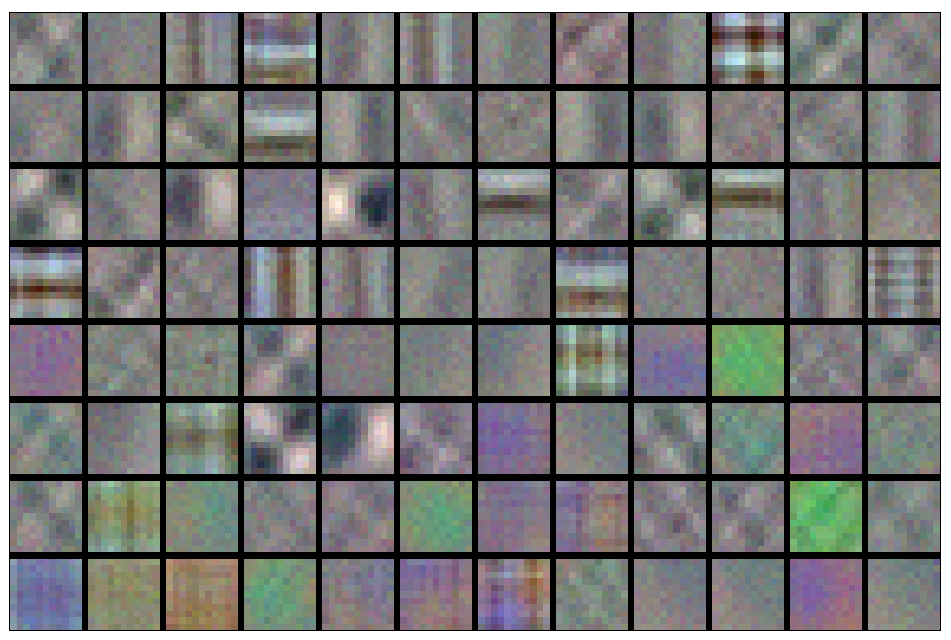
\includegraphics[scale=0.10]{images/l1_filters_iter5000.png}} \hspace{2mm}
\subfloat[15K Iterations]{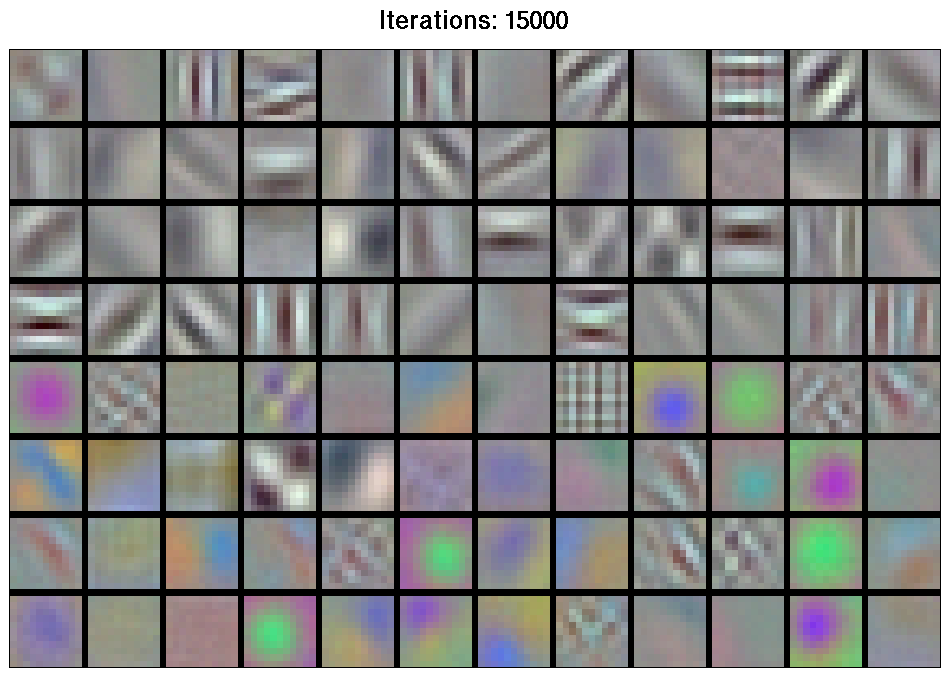
\includegraphics[scale=0.10]{images/l1_filters_iter15000.png}} \hspace{2mm}
\subfloat[305K Iterations]{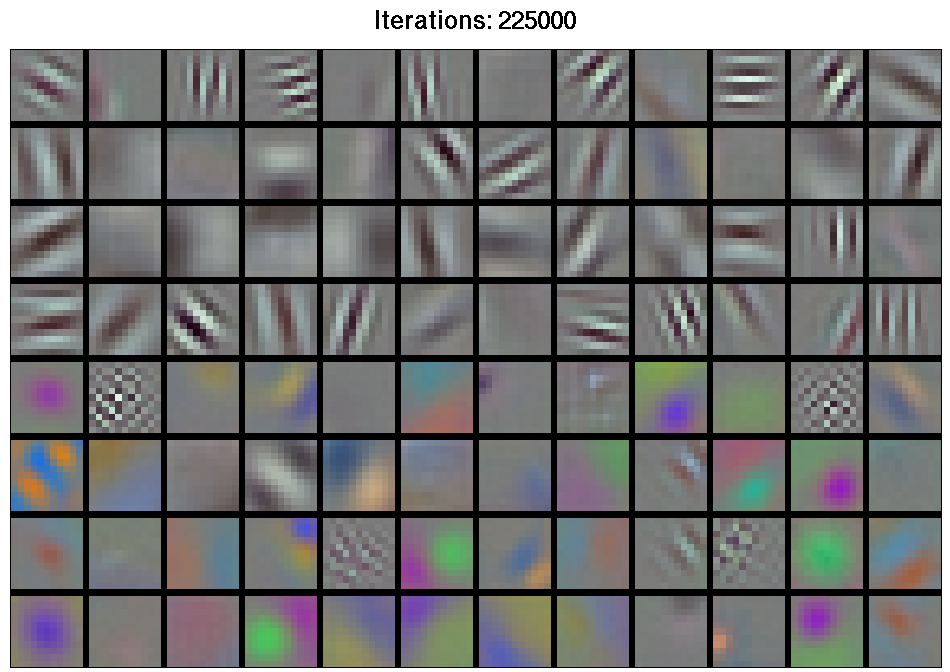
\includegraphics[scale=0.10]{images/l1_filters_iter225000.png}}
\caption{(a),(b),(c) show conv-1 filters after 5K, 15K and 305K iterations of training respectively. One pass (epoch) over the entire Imagenet-ILSVRC12 dataset takes approximately 5K iterations. Notice, that just after 15K iterations these filters closely resemble their final state.}
\begin{comment} Note: I have labeled 305K as 225K - I cannot get the same shape as of the 5K,15K for 305K. The filters look very similar and visually indistiguishable from 305K. If I have time later, I will make them all uniform.
\end{comment}
\label{fig:conv1}
\end{figure}


\setlength{\tabcolsep}{1pt}
\begin{table}[t!]
\begin{center}
\caption{Performance of 50-50 network for detection on pascal-voc-2007 challenge. (l5 is conv-5 and l7 is fc-7)}
\label{table:det-trajectory}
\scalebox{1.00}{
\begin{tabular}{|l|cccc|}
\hline
 & 50K & 105K & 205K & 305K \\
\hline
PASCAL-DET & 50.2 & 52.6 & 55.3 & 55.4 \\
SUN-CLS & 52.8 & 54.7 & 56.4 & 56.6 \\
\hline
\end{tabular}}
\end{center}
\end{table}
\setlength{\tabcolsep}{1.4pt}
The above analysis reinforces our belief that indeed majority of training required for generalization happens quite quickly as compared to the full training time of the network. This observation suggest that there may exist clever ways which can help us speed up the training.




\section{Conclusion}
\label{sec:conclusion}
In this paper we analysed different properties of convolutional neural networks with the aim of gaining insights required to efficiently exploit the rich feature hierarchies provided by such networks. \\

\noindent \textbf{Acknowledgements}
We thank NVIDIA for donating GPUs. We thank Bharath Hariharan, Saurabh Gupta and Joao Carreira for the discussions and helpful suggestions. Pulkit Agrawal is supported on Fulbright Science and Technology fellowship.  

\begin{align}
  \psi (u) & = \int_{0}^{T} \left[\frac{1}{2}
  \left(\Lambda_{0}^{-1} u,u\right) + N^{\ast} (-u)\right] dt \; \\
& = 0 ?
\end{align}


\bibliographystyle{splncs03}
\bibliography{egbib}
\end{document}
